


\chapter{Quantifying multi-structures}\label{chapter:quantifying_multi-structures}

\section{Introduction}

Here, the actual shape and arrangement of multi-structures will be quantified through the use of numbers, or lists of numbers. Before this can be properly done however, the multi-structures will need to be ``smoothed out", so that their ``structure" at extremely small ``{\bf infinitesimal}" scales is uniform and bereft of ``sharp" boundaries.

\section{The smoothness condition}

To ensure that the structure of multi-points remain uniform at infinitesimal scales, each point will be envisioned as a ``cloud" of an infinite number of points, each with an infinitely small, {\bf infinitesimal} weight. When the zoom is increased to infinite scales, the point resembles a cloud of points with the highest density at the center, rapidly dropping of to \(0\) further from the center. Further increases to the scale result in a uniform spread of an infinite number of points each with an infinitesimal weight. By doing this, points have a ``soft/smooth" boundary. This smoothing is illustrated below:

\begin{center}
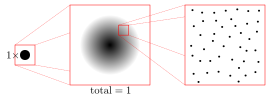
\includegraphics[width = \textwidth]{Smoothness_and_duality/point_smoothing}
\end{center}

To ensure that the structure of multi-paths remain uniform at infinitesimal scales, each path will be envisioned as a ``bundle" of an infinite number of paths, each with an infinitely small, infinitesimal weight. When the zoom is increased to infinite scales, the path resembles a bundle of paths with the highest density at the center, rapidly dropping of to \(0\) further from the center. Further increases to the scale result in a uniform spread of an infinite number of paths each with an infinitesimal weight. By doing this, paths have a ``soft/smooth" boundary. This smoothing is illustrated below:

\begin{center}
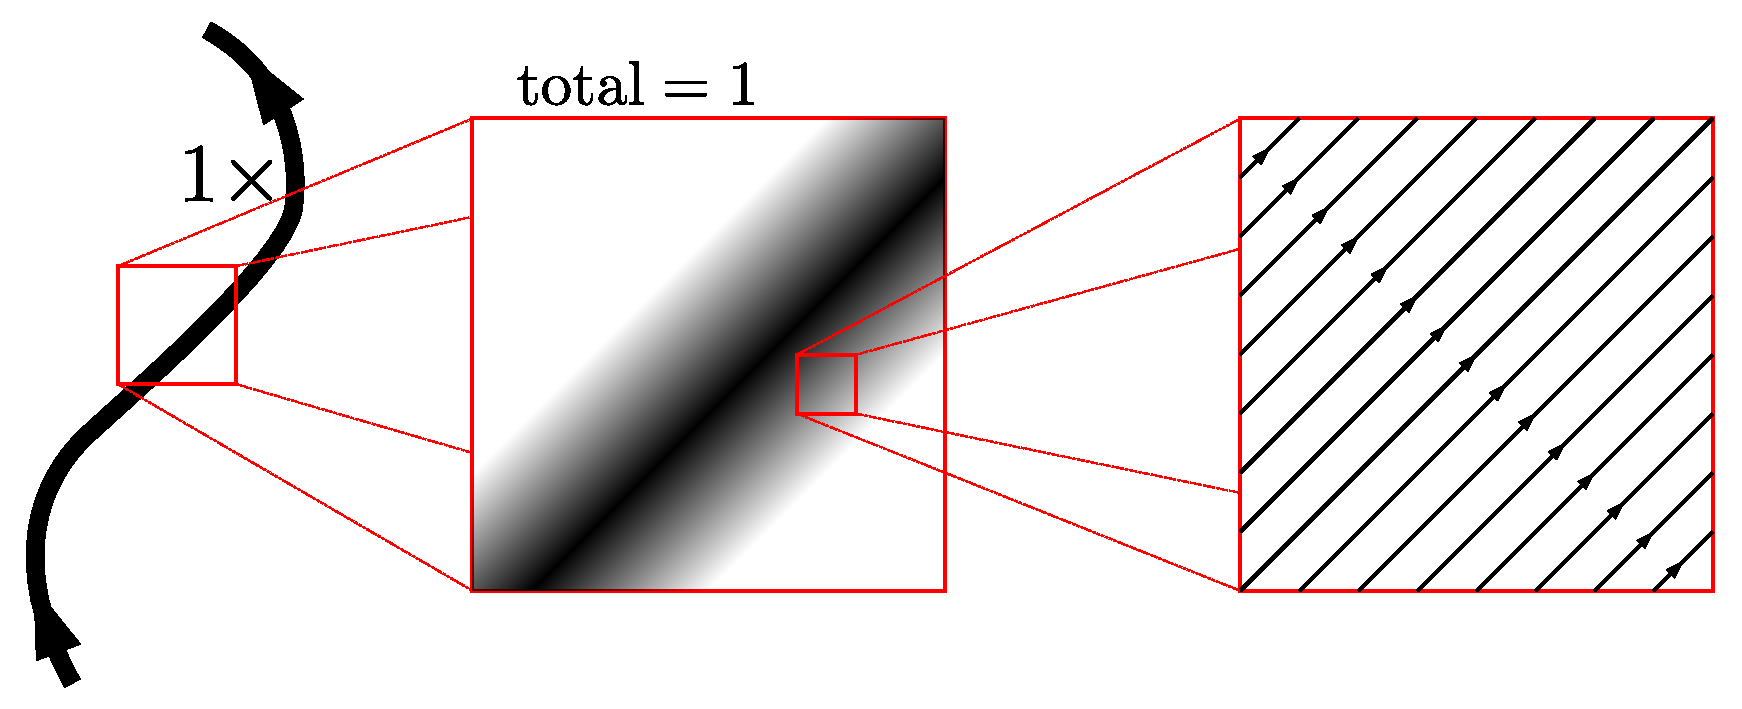
\includegraphics[width = 0.75\textwidth]{Smoothness_and_duality/path_smoothing}
\end{center}

To ensure that the structure of multi-surfaces remain uniform at infinitesimal scales, each surface will be envisioned as a ``stack" of an infinite number of surfaces, each with an infinitely small, infinitesimal weight. When the zoom is increased to infinite scales, the surface resembles a stack of surfaces with the highest density at the center, rapidly dropping of to \(0\) further from the center. Further increases to the scale result in a uniform spread of an infinite number of surfaces each with an infinitesimal weight. By doing this, surfaces have a ``soft/smooth" boundary. This smoothing is illustrated below:

\begin{center}
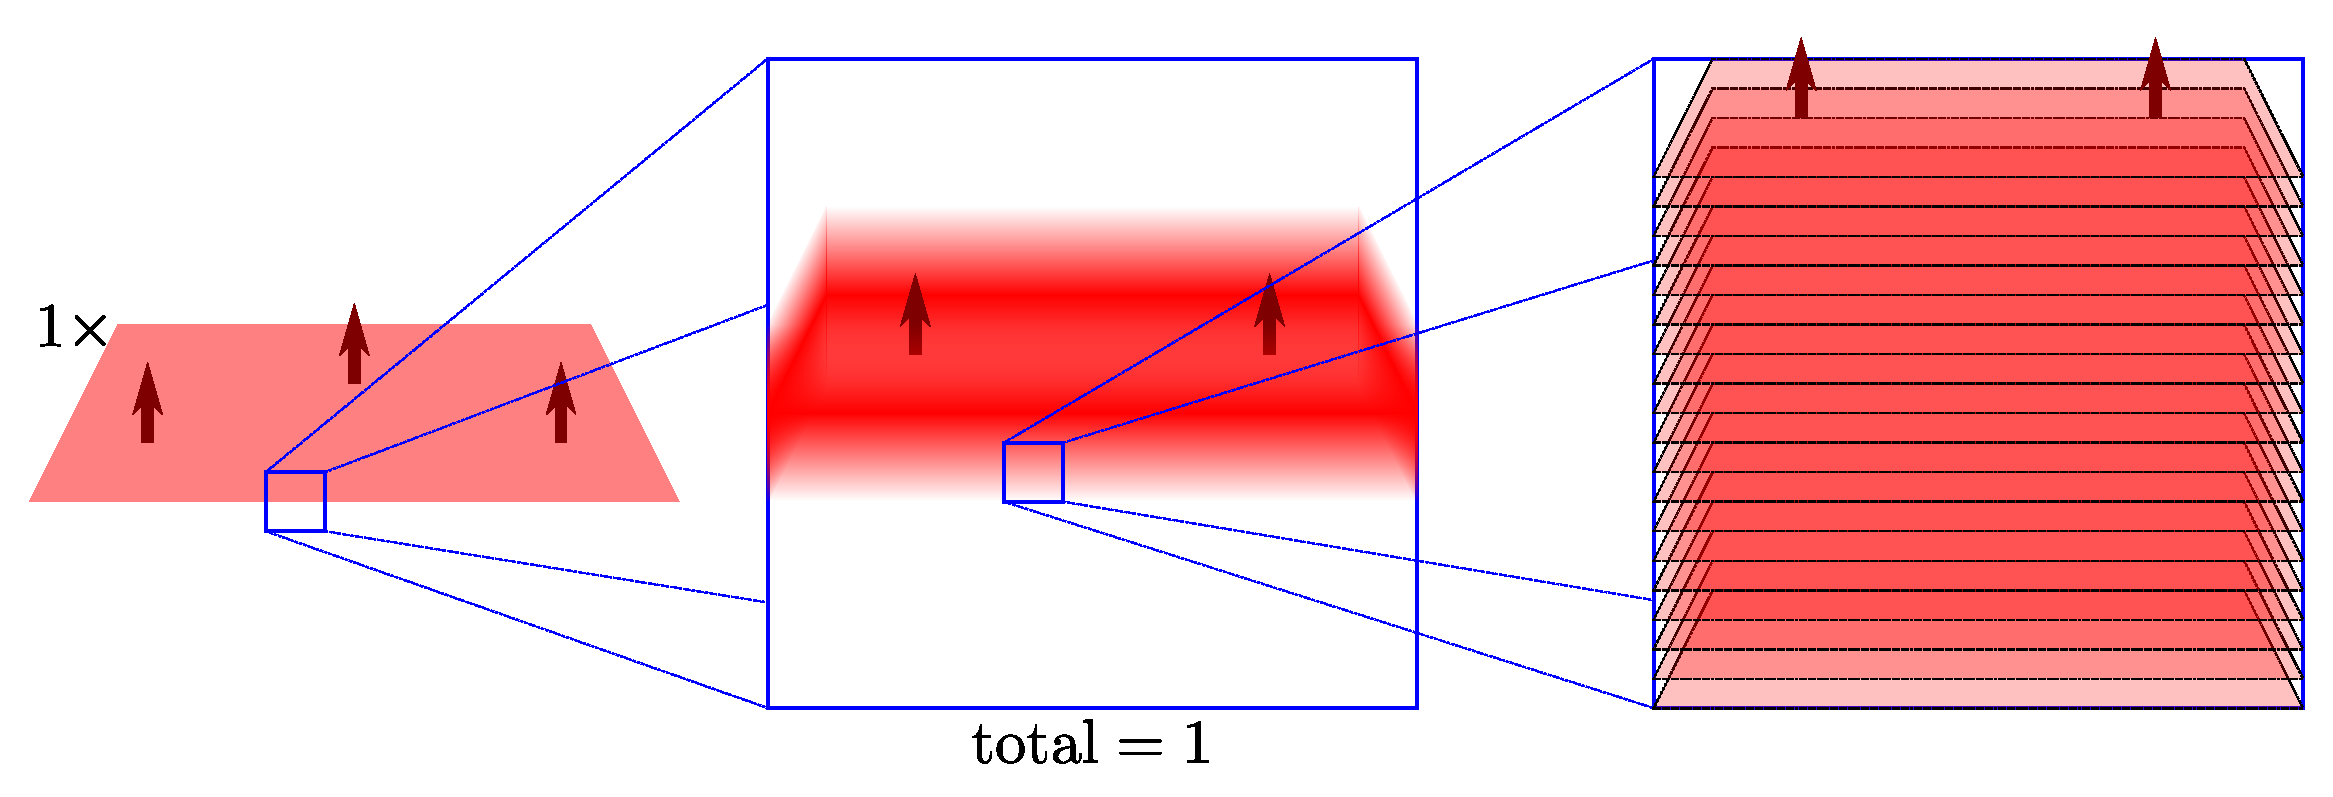
\includegraphics[width = 0.75\textwidth]{Smoothness_and_duality/surface_smoothing}
\end{center}

Lastly, volumes are ``smoothed" by blurring their boundaries at an infinitesimal scale. Each volume is given an infinitely thin ``crust" that consists of onion-like layers of diminishing weight closer to the outside. Essentially, the volume's surface itself is being smoothed as discussed above. This smoothing is illustrated below:

\begin{center}
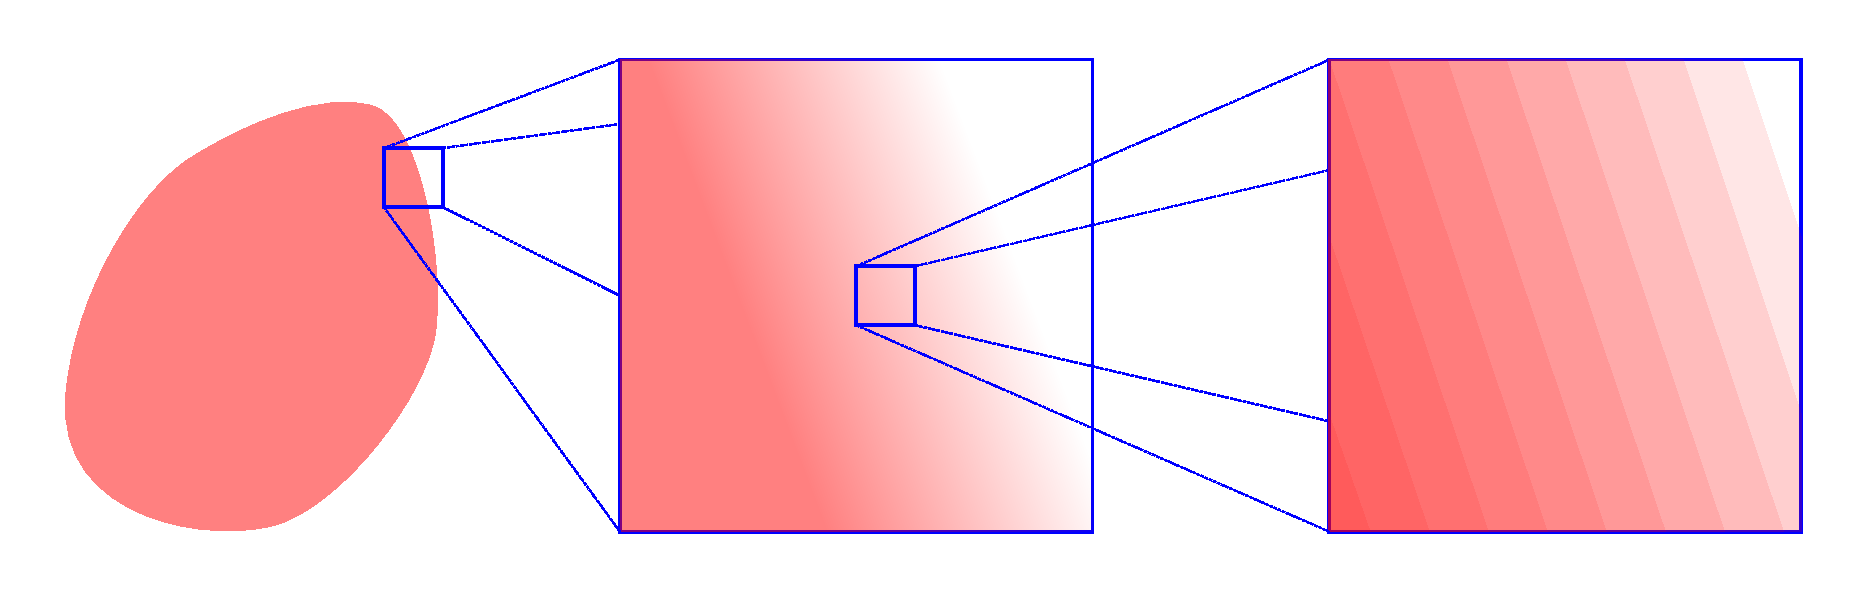
\includegraphics[width = 0.75\textwidth]{Smoothness_and_duality/volume_smoothing}
\end{center}



\section{Unions revisited}

Now that the smoothness requirements on multi-points, multi-paths, multi-surfaces, and multi-volumes have been established, the addition/union of multi-structures now needs to be reconsidered in order to preserve the smoothness requirement. Unions function almost identically to how they functioned previously, but now subtle post-union modifications are made at infinitesimal scales in order to preserve smoothness.  

Below is depicted the union of two clouds of infinitesimally weighted points. The magnification factor is infinite, and after the union, points are moved to ``annihilate" with nearby points with the opposite polarity. 

\begin{center}
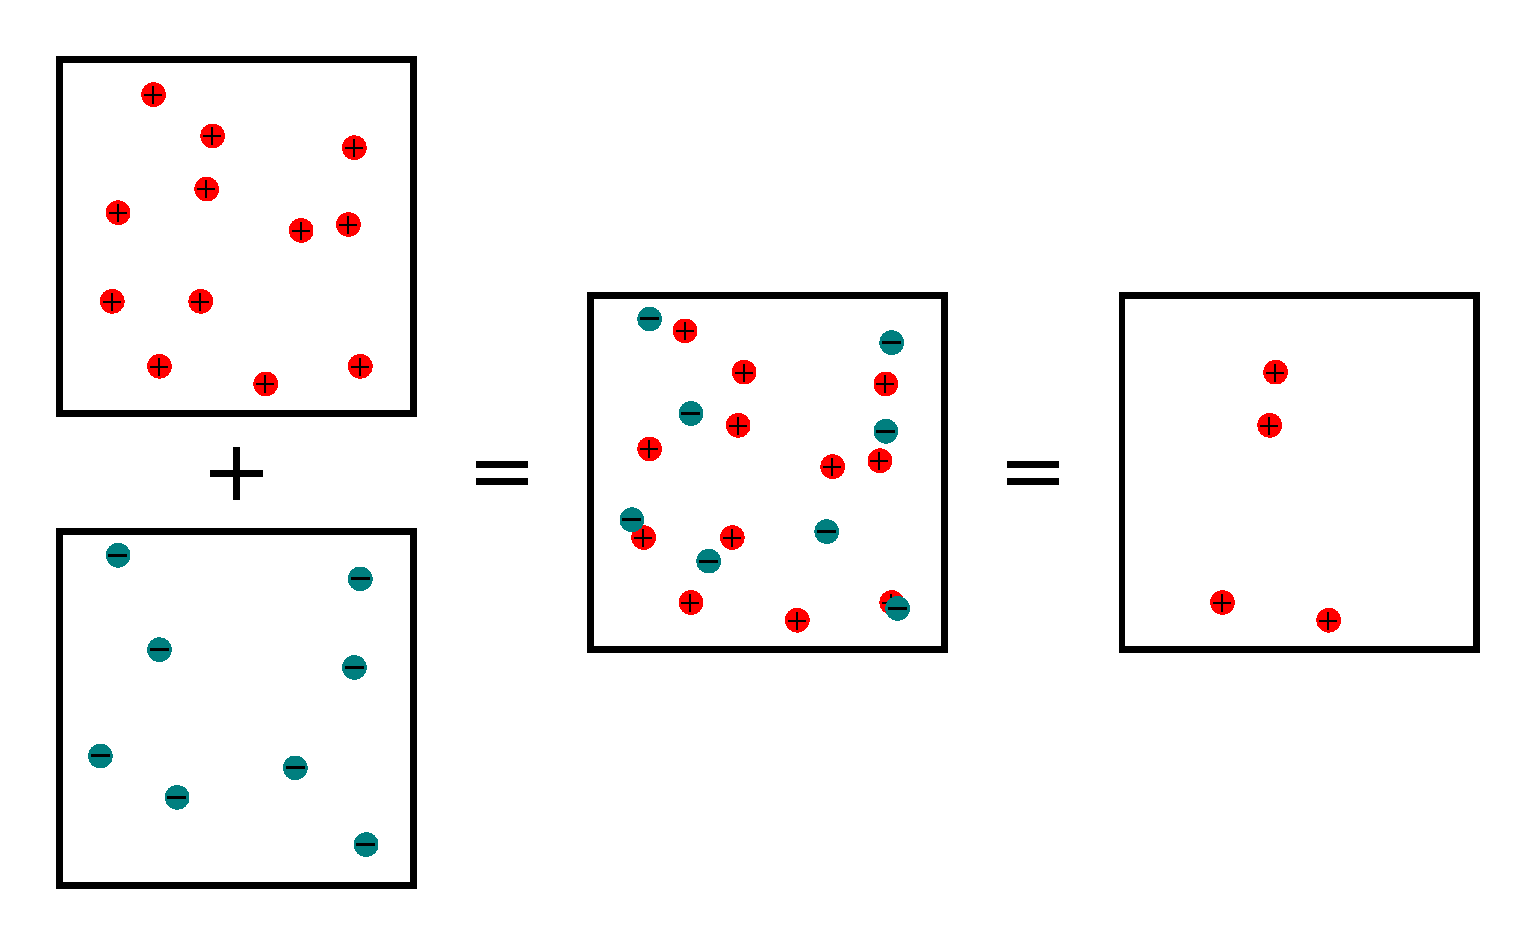
\includegraphics[width = 0.6\textwidth]{Smoothness_and_duality/point_union_smoothing}
\end{center}

Below is depicted the union of two bundles of infinitesimally weighted paths. One bundle is red in color, and the other is green in color. The magnification factor is infinite, and after the union, the paths are broken apart and restitched together into a bundle of ``zigzags", that all have roughly the same overall direction. The zigzags are then ironed out to form a bundle of parallel paths, which is the smoothed union.

\begin{center}
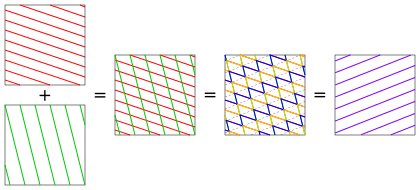
\includegraphics[width = 0.8\textwidth]{Smoothness_and_duality/path_union_smoothing}
\end{center}

\begin{tabular}{cc}
\parbox{0.5\textwidth}{
To the right is depicted the union of two stacks of infinitesimally weighted surfaces, which proceeds in a virtually identical manner to the union of paths. One stack is red in color, and the other is green in color. The magnification factor is infinite, and after the union, the surfaces are broken apart and restitched together into a stack of corrugated surfaces. The corrugated surfaces are then ironed out to form the stack of blue parallel surfaces, which is the smoothed union.
} & \parbox{0.5\textwidth}{
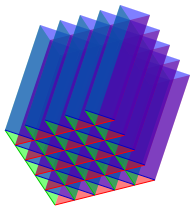
\includegraphics[width = 0.5\textwidth]{Smoothness_and_duality/surface_union_smoothing}
}
\end{tabular}

Lastly, when the union of two multi-volumes occurs, the surfaces of the sum need to be smoothed out in a manner similar to what was described above.

{\bf It is important to note that smoothing does not impact any of the properties regarding unions, intersections, and boundaries that were mentioned in the previous chapters.}





\section{Coordinate systems}

\begin{tabular}{cc}
\parbox{0.5\textwidth}{
A coordinate system labels each point with a triple of numbers \((c_1, c_2, c_3)\). On the right, a ``coordinate lattice" is depicted where each point in the lattice is determined by a unique triple \((c_1, c_2, c_3)\). Changing one coordinate while holding the others constant moves the point along one of the lattice lines. Principal direction \(i\) is the direction of the line traced out by increasing \(c_i\).

The coordinate system will be assumed to be {\bf right handed}. With both the \(c_1\) and \(c_2\) directions oriented upwards, and the \(c_1\) direction is on your left, the \(c_2\) direction on your right, then the \(c_3\) direction is oriented away from the viewer.

Some important notation to keep track of is as follows: The coordinates are indexed from \(1\) to \(3\). If variable \(i\) {\bf denotes an index} with the range \(1, 2, 3\), then the expression \(i + 1\) adds \(1\) to index \(i\) while {\bf wrapping the values around} so that increasing from \(3\) returns to \(1\): \(3 + 1 = 1\). The expression \(i + 2\) adds \(2\) to index \(i\) while {\bf wrapping the values around} so that increasing from \(3\) returns to \(1\): \(2 + 2 = 1\) and \(3 + 2 = 2\). Given an index \(i\), the {\bf other indices} are \(i+1\) and \(i+2\).
} & \parbox{0.5\textwidth}{
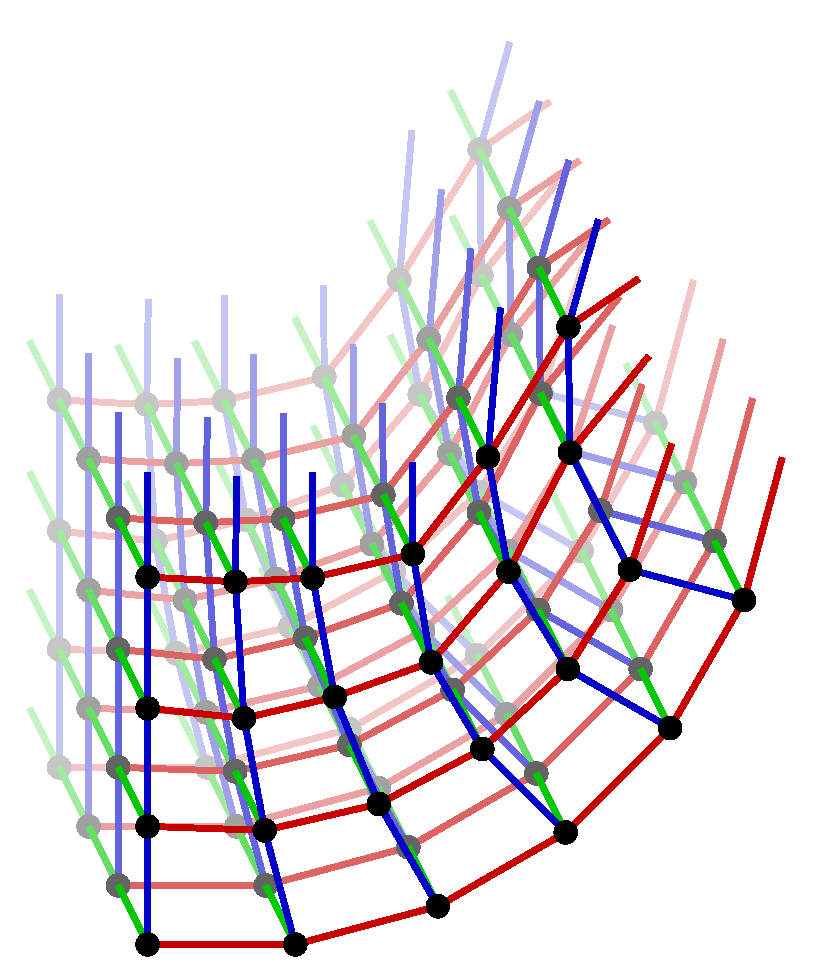
\includegraphics[width = 0.5\textwidth]{Coordinate_systems/coordinate_system_lattice}
}
\end{tabular}

\vspace{1mm}

The coordinate values \(c_1\), \(c_2\), and \(c_3\) may not be dimensionless and may instead have units of measurement. For example, with Cartesian coordinates, all coordinates are measured using units of length. The units that measure \(c_1\), \(c_2\), and \(c_3\) will be denoted by ``c\_1\_units"; ``c\_2\_units"; and ``c\_3\_units" respectively. 

A \textbf{vector} is a {\bf list of numbers}. Vectors are often denoted by listing their numbers vertically within square braces, or horizontally within triangular braces: 
\[\begin{bmatrix} F_1 \\ F_2 \\ \vdots \\ F_n \end{bmatrix} \quad\text{or}\quad \langle F_1, F_2, ..., F_n \rangle\]
If the entries of a vector are computed via the expression \(F(i)\), where \(i\) (from the range \(1, 2, ..., n\)) is the index of the entry being computed, then the vector itself is denoted via the expression \([i : F(i)]\) or \(\langle i : F(i) \rangle\).

Lastly, given an expression \(F(i)\) where \(i\) is an index from the range \(1, 2, ..., n\), then \(\sum_i F(i)\) denotes the sum \(F(1) + F(2) + ... + F(n)\).

\vspace{1mm}

\begin{tabular}{cc}
\parbox{0.5\textwidth}{
A {\bf parallelepiped} is the 3D analog to the parallelogram. When the coordinates \(c_1\), \(c_2\), and \(c_3\) are changed by the respective infinitesimal (infinitely small) amounts \(\Delta c_1\), \(\Delta c_2\), and \(\Delta c_3\), the set of all points where \(c_1\), \(c_2\), and \(c_3\) are in between their old and new values is approximately a parallelepiped, such as depicted on the right. The various dimensions of this parallelepiped are proportional to \(\Delta c_1\), \(\Delta c_2\), and \(\Delta c_3\). 
} & \parbox{0.5\textwidth}{
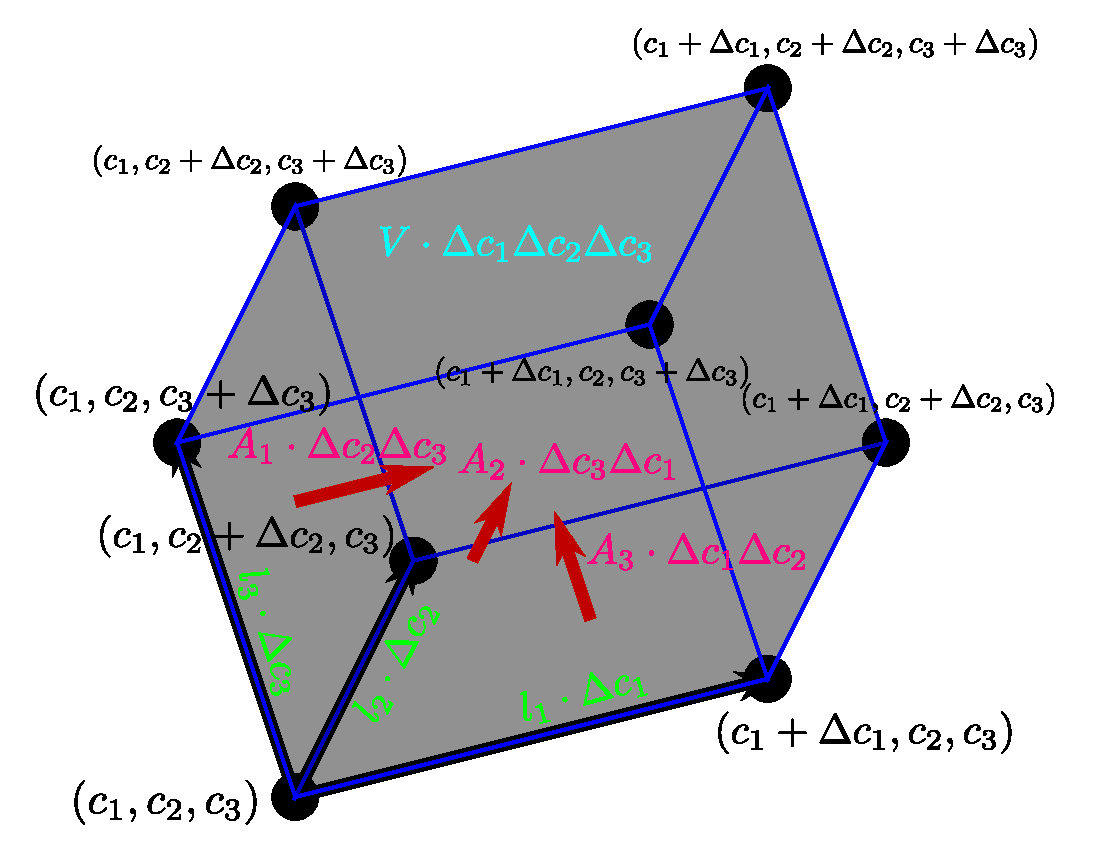
\includegraphics[width = 0.5\textwidth]{Coordinate_systems/coordinate_system_cell}
}
\end{tabular}

\vspace{1mm}

For each dimension \(i = 1, 2, 3\), when coordinate \(c_i\) changes by the infinitesimal amount \(\Delta c_i\), the point moves a distance of \(l_i \cdot \Delta c_i\). The quantity \(l_i\) is the distance traversed by the point per unit of \(c_i\) (for infinitesimal changes in \(c_i\)). {\bf Principal direction} \(i\) is the direction of the edge traced out by increasing \(c_i\). The values of \(l_1\), \(l_2\), and \(l_3\) are measured using the following respective units: \(\text{m}/\text{c\_1\_units}\), \(\text{m}/\text{c\_2\_units}\), and \(\text{m}/\text{c\_3\_units}\).   

For each dimension \(i = 1, 2, 3\), when the other coordinates \(c_{i+1}\) and \(c_{i+2}\) change by the respective infinitesimal amounts \(\Delta c_{i+1}\) and \(\Delta c_{i+2}\), the area of the parallelogram formed by all points where \(c_{i+1}\) and \(c_{i+2}\) are in between their old and new values is \(A_i \cdot \Delta c_{i+1} \Delta c_{i+2}\). {\bf Co-principal direction} \(i\) is the direction perpendicular to this parallelogram (illustrated by the red arrows). The values of \(A_1\), \(A_2\), and \(A_3\) are measured using the following respective units: \(\text{m}^2/(\text{c\_2\_units} \cdot \text{c\_3\_units})\), \(\text{m}^2/(\text{c\_3\_units} \cdot \text{c\_1\_units})\), and \(\text{m}^2/(\text{c\_1\_units} \cdot \text{c\_2\_units})\).     

Lastly when all coordinates \(c_1\), \(c_2\), and \(c_3\) change by the respective infinitesimal amounts \(\Delta c_1\), \(\Delta c_2\), and \(\Delta c_3\), the volume of the parallelepiped (3D parallelogram) formed by all points where \(c_1\), \(c_2\), and \(c_3\) are in between their old and new values is \(V \cdot \Delta c_1 \Delta c_2 \Delta c_3\). The value of \(V\) is measured using the units: \(\text{m}^3/(\text{c\_1\_units} \cdot \text{c\_2\_units} \cdot \text{c\_3\_units})\) 

\begin{tabular}{cc}
\parbox{0.5\textwidth}{
In addition to the quantities \(l_1\), \(l_2\), \(l_3\), \(A_1\), \(A_2\), \(A_3\), and \(V\), additional quantities will be introduced. For each \(i = 1, 2, 3\), \(B_i \cdot \Delta c_{i+1} \Delta c_{i+2}\) is the cross-sectional area when the parallelepiped is cleaved perpendicular to the \(c_i\) direction, and \(h_i \cdot \Delta c_i\) is the thickness/height of the parallelepiped when placed flat along the \(c_{i+1}\) and \(c_{i+2}\) directions. All of these quantities are illustrated on the right. For simplicity, the factors \(\Delta c_1\), \(\Delta c_2\), and \(\Delta c_3\) have been omitted. \(h_1\), \(h_2\), and \(h_3\) have the same units of measurement as \(l_1\), \(l_2\), and \(l_3\) respectively. \(B_1\), \(B_2\), and \(B_3\) have the same units of measurement as \(A_1\), \(A_2\), and \(A_3\) respectively.  

The relationship between these quantities, derived from computing the volume in multiple different ways, are:
\begin{align*}
V = & l_1 B_1 = l_2 B_2 = l_3 B_3 \\ 
= & h_1 A_1 = h_2 A_2 = h_3 A_3
\end{align*} 
} & \parbox{0.5\textwidth}{
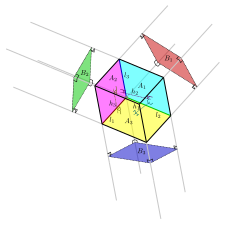
\includegraphics[width = 0.5\textwidth]{Coordinate_systems/coordinate_system}
}
\end{tabular}

All of the quantities \(l_1\), \(l_2\), \(l_3\), \(A_1\), \(A_2\), \(A_3\), \(V\), \(B_1\), \(B_2\), \(B_3\), \(h_1\), \(h_2\), and \(h_3\) {\bf may change with respect to position}.

To assist in describing multi-structures and computing various quantities, space will be broken in a lattice of ``cells". Infinitesimal increments \(\Delta c_1\), \(\Delta c_2\), and \(\Delta c_3\) will be fixed. For any choice of {\bf integers} \(k_1\), \(k_2\), and \(k_3\), the {\bf cell} indexed by the triple \((k_1, k_2, k_3)\) is the parallelepiped where for each index \(i = 1, 2, 3\), that coordinate \(c_i\) is confined to the narrow interval \(k_i \Delta c_i \leq c_i < (k_i + 1)\Delta c_i\). Note that the upper bound on the interval is excluded. 

\vspace{1mm}

\begin{tabular}{cc}
\parbox{0.4\textwidth}{
Point \(\theta_{(k_1, k_2, k_3)}\) is a lattice note with the coordinate \((k_1 \Delta c_1, k_2 \Delta c_2, k_3 \Delta c_3)\). 

\vspace{1mm}

For each index \(i = 1, 2, 3\); \(\alpha_{i, (k_1, k_2, k_3)}\) is the lattice curve/edge that consists of all points where \(c_i\) increases from \(k_i \Delta c_i\) to \((k_i + 1)\Delta c_i\) and the other coordinates are held constant: \(c_{i+1} = k_{i+1} \Delta c_{i+1}\) and \(c_{i+2} = k_{i+2} \Delta c_{i+2}\). This curve starts at \(\theta_{(k_1, k_2, k_3)}\) and does not include the end point where \(c_i = (k_i + 1)\Delta c_i\).

\vspace{1mm}

For each index \(i = 1, 2, 3\); \(\sigma_{i, (k_1, k_2, k_3)}\) is the lattice surface/tile that consists of all points where \(c_i = k_i \Delta c_i\) and \(k_{i+1} \Delta c_{i+1} \leq c_{i+1} < (k_{i+1} + 1) \Delta c_{i+1}\) and \(k_{i+2} \Delta c_{i+2} \leq c_{i+2} < (k_{i+2} + 1) \Delta c_{2+1}\). The surface faces in the direction of increasing \(c_i\) and does not include the points where \(c_{i+1} = (k_{i+1} + 1)\Delta c_{i + 1}\) or \(c_{i+2} = (k_{i+2} + 1)\Delta c_{i + 2}\).
} & \parbox{0.6\textwidth}{
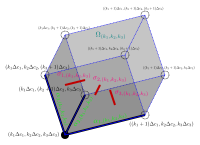
\includegraphics[width = 0.6\textwidth]{Coordinate_systems/coordinate_system_cell_2}
}
\end{tabular}

\vspace{1mm}

\(\Omega_{(k_1, k_2, k_3)}\) is the cell itself. Note that points where \(c_1 = (k_1 + 1)\Delta c_1\) or \(c_2 = (k_2 + 1)\Delta c_2\) or \(c_3 = (k_3 + 1)\Delta c_3\) are not included.

Associated with each cell are the aforementioned quantities \(l_1\), \(l_2\), \(l_3\), \(A_1\), \(A_2\), \(A_3\), \(V\), \(B_1\), \(B_2\), \(B_3\), \(h_1\), \(h_2\), and \(h_3\). {\bf These quantities may change from cell to cell.}




\section{Using numbers to describe multi-structures}

Multi-structures will be denoted by functions whose input is a point and space, and whose return values are numbers that describe the total-multi structure at that point. Given an arbitrary point \((c_1, c_2, c_3)\), the indices \((k_1, k_2, k_3)\) of the cell that contains \((c_1, c_2, c_3)\) are:
\[(k_1, k_2, k_3) = \left(\left\lfloor\frac{c_1}{\Delta c_1}\right\rfloor, \left\lfloor\frac{c_2}{\Delta c_2}\right\rfloor, \left\lfloor\frac{c_3}{\Delta c_3}\right\rfloor\right)\] 
The notation \(\lfloor x \rfloor\) means to round \(x\) \emph{down} to the nearest integer provided \(x\) is not an integer. If \(x\) is already an integer \(\lfloor x \rfloor = x\). 

{\bf The first step in quantifying a multi-structure is to ``approximate" the multi-structure using \emph{only} the lattice nodes \(\theta\) for multi-points, the lattice edges \(\alpha_i\) for multi-paths, the lattice tiles \(\sigma_i\) for multi-surfaces, and the lattice cells \(\Omega\) for multi-volumes.} 


\subsection{Quantifying multi-points}

A multi-point \(\rho\) is quantified by a function \(\rho(\mathbf{q})\) whose input is a position \(\mathbf{q}\). 

\begin{tabular}{cc}
\parbox{0.5\textwidth}{
Let triple \((k_1, k_2, k_3)\) index the cell that contains \(\mathbf{q}\). At the scales of \(\Delta c_1\), \(\Delta c_2\), and \(\Delta c_3\), the magnification results in the points resembling a uniform spread of infinitesimal points thanks to the smoothness condition, as depicted in the leftmost image on the right. The approximation takes the total point weight inside the cell and condenses it onto the lattice point \(\theta_{(k_1,k_2,k_3)}\), as depicted in the rightmost image on the right. {\bf This is the approximation that will be used for various calculations.}
} & \parbox{0.5\textwidth}{
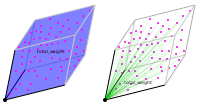
\includegraphics[width = 0.5\textwidth]{Coordinate_systems/point_density}
}
\end{tabular}

What about the value of \(\rho(\mathbf{q})\) itself? The weight \(w_\theta\) assigned to the lattice point \(\theta_{(k_1,k_2,k_3)}\) is infinitely small, so the average density over the cell volume is used for \(\rho(\mathbf{q})\) instead: \(\rho(\mathbf{q}) = \frac{w_\theta}{V \cdot \Delta c_1 \Delta c_2 \Delta c_3}\). Contrariwise, if \(\rho(\mathbf{q})\) is known, then the weight assigned to \(\theta_{(k_1,k_2,k_3)}\) is \(\rho(\mathbf{q}) \cdot V \cdot \Delta c_1 \Delta c_2 \Delta c_3\). In essence, \(\rho(\mathbf{q})\) is the point weight density.

If length is being measured in meters (m), and weight is being measured using an arbitrary unit of measurement referred to as ``w\_units", then the value of \(\rho(\mathbf{q})\) is measured in \(\text{w\_units}/\text{m}^3\) (i.e. w\_units per unit volume).




\subsection{Quantifying multi-paths}

A multi-path \(\mathbf{J}\) is quantified by a vector valued function \(\mathbf{J}(\mathbf{q}) = [i : J_i(\mathbf{q})] = \begin{bmatrix} J_1(\mathbf{q}) \\ J_2(\mathbf{q}) \\ J_3(\mathbf{q}) \end{bmatrix}\) whose input is a position \(\mathbf{q}\). 

\begin{tabular}{cc}
\parbox{0.5\textwidth}{
Let triple \((k_1, k_2, k_3)\) index the cell that contains \(\mathbf{q}\). At the scales of \(\Delta c_1\), \(\Delta c_2\), and \(\Delta c_3\), the magnification results in the paths resembling a uniform bundle of infinitesimally weighted paths thanks to the smoothness condition. For each direction \(i = 1, 2, 3\), the total weight of all of the intersections with the lattice tile \(\sigma_{i, (k_1, k_2, k_3)}\) is the total path weight that crosses the current cell in principal direction \(i\), and this total weight is subsequently assigned to the lattice edge \(\alpha_{i, (k_1, k_2, k_3)}\) which itself crosses the current cell in principal direction \(i\). {\bf This is the approximation that will be used for various calculations.} 
} & \parbox{0.5\textwidth}{
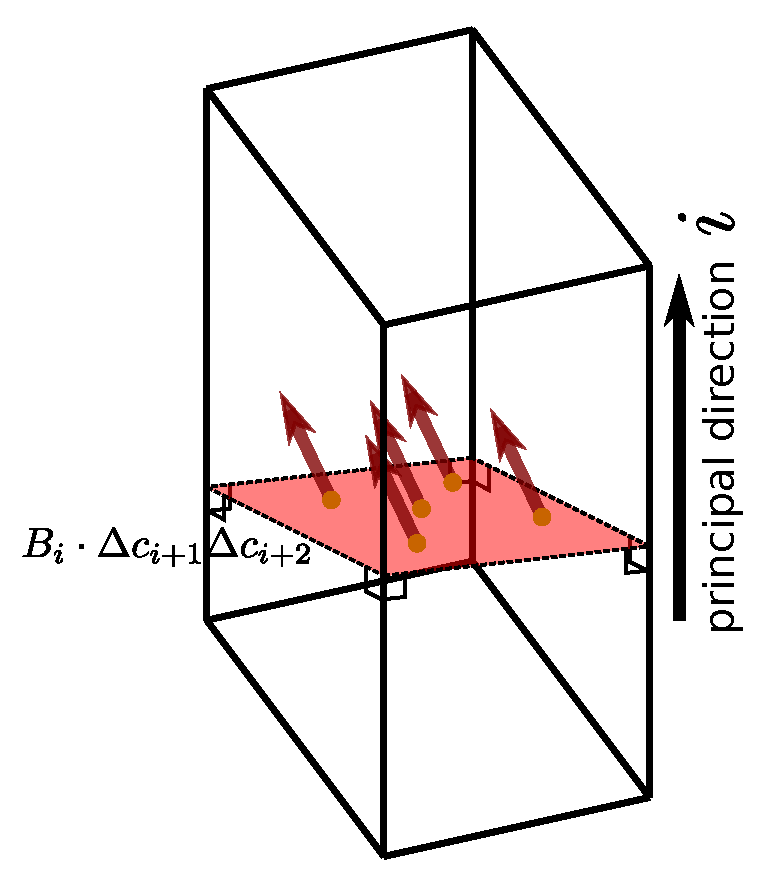
\includegraphics[width = 0.5\textwidth]{Coordinate_systems/path_density}
}
\end{tabular}

What about the value of \(J_i(\mathbf{q})\) itself? The weight \(w_{\alpha,i}\) assigned to the lattice edge \(\alpha_{i, (k_1,k_2,k_3)}\) is infinitely small, so the average density over the cross-sectional area of the cell is used for \(J_i(\mathbf{q})\) instead: \(J_i(\mathbf{q}) = \frac{w_{\alpha,i}}{B_i \cdot \Delta c_{i+1} \Delta c_{i+2}}\). Contrariwise, if \(J_i(\mathbf{q})\) is known, then the weight assigned to \(\alpha_{i, (k_1,k_2,k_3)}\) is \(J_i(\mathbf{q}) \cdot B_i \cdot \Delta c_{i+1} \Delta c_{i+2}\).

If length is being measured in meters (m), and weight is being measured using an arbitrary unit of measurement referred to as ``w\_units", then the values of \(\mathbf{J}(\mathbf{q})\) are measured in \(\text{w\_units}/\text{m}^2\) (i.e. w\_units per unit cross sectional area).

%To assist in visualizing multi-paths for the purpose or computing various quantities, the multi-paths will be ``roughened" and then broken apart and reassembled into paths that aree parallel to the principal directions, in exactly the reverse of the ``smoothing" that takes place after the union of two multi-paths is computed:
%
%\begin{center}
%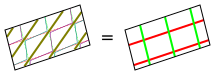
\includegraphics[width = 0.8\textwidth]{Coordinate_systems/2D_multi-path_breakdown}
%\end{center}
%
%For each \(i = 1, 2, 3\), \(J_i(\mathbf{q}) \cdot B_i \cdot \Delta c_{i+1} \Delta c_{i+2}\) is the total weight of the paths parallel to the \(i^{\text{th}}\) principal direction.




\subsection{Quantifying multi-surfaces}

A multi-surface \(\mathbf{F}\) is quantified by a vector valued function \(\mathbf{F}(\mathbf{q}) = [i : F_i(\mathbf{q})] = \begin{bmatrix} F_1(\mathbf{q}) \\ F_2(\mathbf{q}) \\ F_3(\mathbf{q}) \end{bmatrix}\) whose input is a position \(\mathbf{q}\). 

\vspace{5mm}

\begin{tabular}{cc}
\parbox{0.5\textwidth}{
Let triple \((k_1, k_2, k_3)\) index the cell that contains \(\mathbf{q}\). At the scales of \(\Delta c_1\), \(\Delta c_2\), and \(\Delta c_3\), the magnification results in the surfaces resembling a uniform stack of infinitesimally weighted surfaces thanks to the smoothness condition. For each direction \(i = 1, 2, 3\), the total weight of all of the intersections with the lattice edge \(\alpha_{i, (k_1, k_2, k_3)}\) is the total surface weight that slices through the current cell blocking direction \(i\), and this total weight is subsequently assigned to the lattice tile \(\sigma_{i, (k_1, k_2, k_3)}\) which itself blocks direction \(i\). {\bf This is the approximation that will be used for various calculations.} 
} & \parbox{0.5\textwidth}{
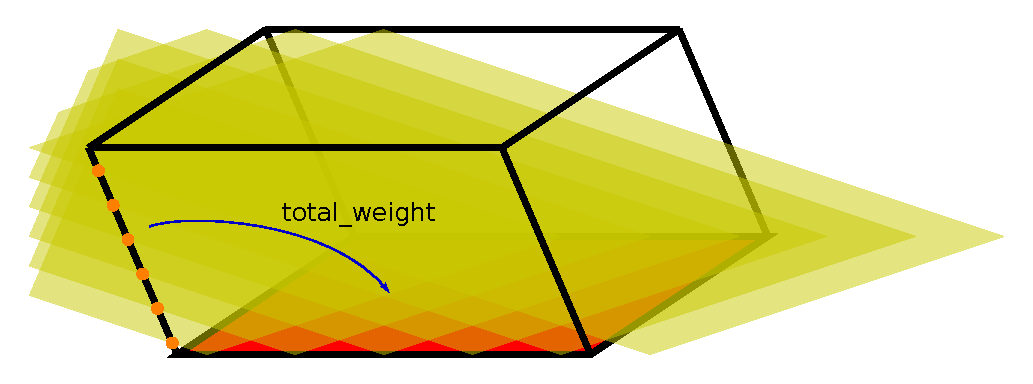
\includegraphics[width = 0.5\textwidth]{Coordinate_systems/surface_density}
}
\end{tabular}

\vspace{5mm}

What about the value of \(F_i(\mathbf{q})\) itself? The weight \(w_{\sigma,i}\) assigned to the lattice tile \(\sigma_{i, (k_1,k_2,k_3)}\) is infinitely small, so the average density over the thickness of the cell is used for \(F_i(\mathbf{q})\) instead: \(F_i(\mathbf{q}) = \frac{w_{\sigma,i}}{h_i \cdot \Delta c_i}\). Contrariwise, if \(F_i(\mathbf{q})\) is known, then the weight assigned to \(\sigma_{i, (k_1,k_2,k_3)}\) is \(F_i(\mathbf{q}) \cdot h_i \cdot \Delta c_i\).

If length is being measured in meters (m), and weight is being measured using an arbitrary unit of measurement referred to as ``w\_units", then the values of \(\mathbf{F}(\mathbf{q})\) are measured in \(\text{w\_units}/\text{m}\) (i.e. w\_units per unit thickness).





\subsection{Quantifying multi-volumes}

A multi-volume \(U\) is quantified by a function \(U(\mathbf{q})\) whose input is a position \(\mathbf{q}\). In earlier sections, \(U(\mathbf{q})\) was defined as the net number of volumes that contain position \(\mathbf{q}\). This definition will remain, but an approximation of \(U\) using the cells \(\Omega_{(k_1, k_2, k_3)}\) will be established. 

For each triple \((k_1, k_2, k_3)\) the weight assigned to cell \(\Omega_{(k_1, k_2, k_3)}\) is the average value of \(U(\mathbf{q})\) for all positions from said cell. This has the effect of ``pixelating" \(U\) using the cells \(\Omega_{(k_1, k_2, k_3)}\), as is depicted below. For all positions \(\mathbf{q}\) in cell \((k_1, k_2, k_3)\), the net number of volumes that contain \(\mathbf{q}\) is approximately the weight \(w_{\Omega}\) assigned to the cell \(\Omega_{(k_1, k_2, k_3)}\): \(U(\mathbf{q}) \approx w_{\Omega}\). {\bf This is the approximation that will be used for various calculations.} 

\begin{center}
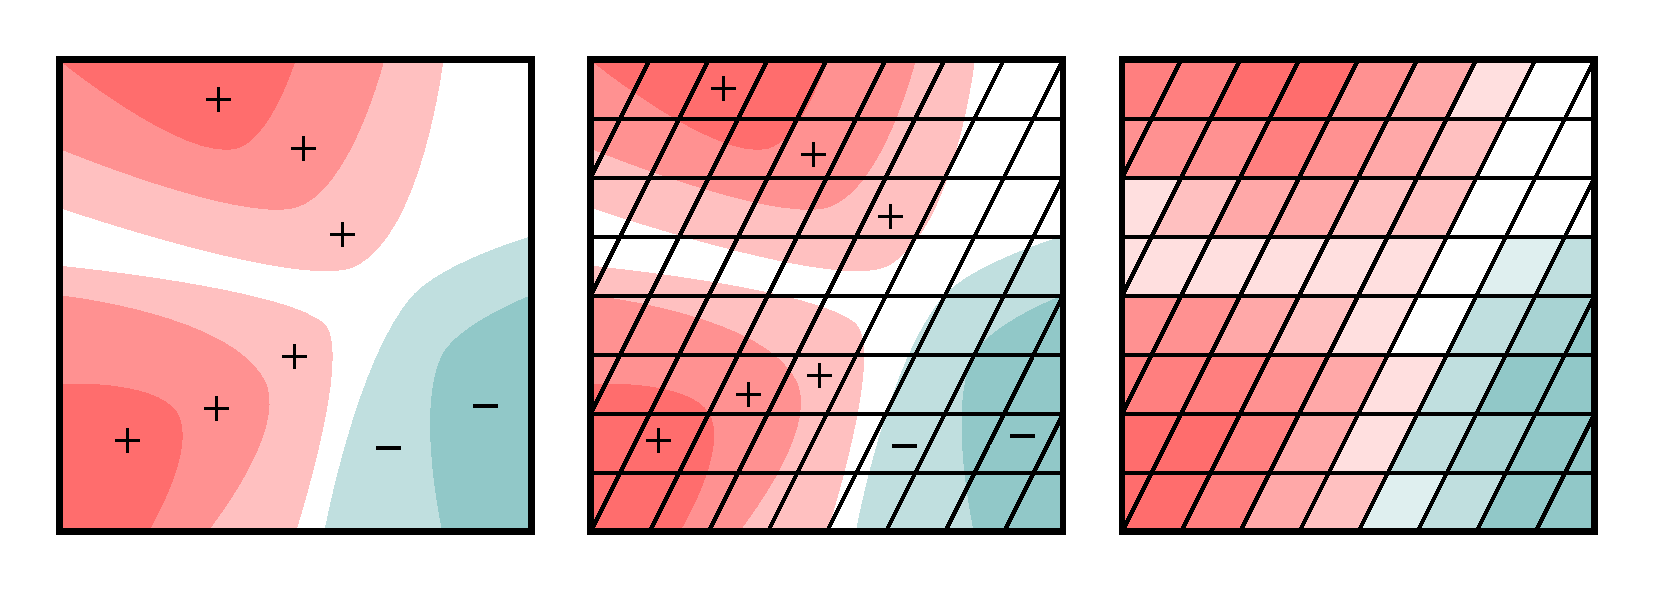
\includegraphics[width = \textwidth]{Coordinate_systems/volume_pixelation}
\end{center}

If length is being measured in meters (m), and weight is being measured using an arbitrary unit of measurement referred to as ``w\_units", then the value of \(U(\mathbf{q})\) is also measured in \(\text{w\_units}\) (no extra dimensions are added).

\vspace{5mm}

{\bf To simplify notation, unless explicitly included, the position parameter \(\mathbf{q}\) will be suppressed in the notation. Be mindful of the various quantities that do change with position.}



\section{Computing unions}

Computing the unions of two multi-structures of the same type is obvious: just add the functions.

\begin{thm}
Given the two multi-points \(\rho\) and \(\mu\), the union is simply the sum of the functions:

\[\rho + \mu = \rho(\mathbf{q}) + \mu(\mathbf{q})\]


Given the two multi-paths \(\mathbf{J} = [i : J_i] = \begin{bmatrix} J_1 \\ J_2 \\ J_3 \end{bmatrix}\) and \(\mathbf{K} = [i : K_i] = \begin{bmatrix} K_1 \\ K_2 \\ K_3 \end{bmatrix}\), the entries of the union is the sum of the corresponding entries from \(\mathbf{J}\) and \(\mathbf{K}\):

\[\mathbf{J} + \mathbf{K} = \begin{bmatrix} J_1 \\ J_2 \\ J_3 \end{bmatrix} + \begin{bmatrix} K_1 \\ K_2 \\ K_3 \end{bmatrix} = \begin{bmatrix} J_1 + K_1 \\ J_2 + K_2 \\ J_3 + K_3 \end{bmatrix} = [i : J_i + K_i]\]


Given the two multi-surfaces \(\mathbf{F} = [i : F_i] = \begin{bmatrix} F_1 \\ F_2 \\ F_3 \end{bmatrix}\) and \(\mathbf{G} = [i : G_i] = \begin{bmatrix} G_1 \\ G_2 \\ G_3 \end{bmatrix}\), the entries of the union is the sum of the corresponding entries from \(\mathbf{F}\) and \(\mathbf{G}\):

\[\mathbf{F} + \mathbf{G} = \begin{bmatrix} F_1 \\ F_2 \\ F_3 \end{bmatrix} + \begin{bmatrix} G_1 \\ G_2 \\ G_3 \end{bmatrix} = \begin{bmatrix} F_1 + G_1 \\ F_2 + G_2 \\ F_3 + G_3 \end{bmatrix} = [i : F_i + G_i]\]


Given the two multi-volumes \(U\) and \(T\), the union is simply the sum of the functions:

\[U + T = U(\mathbf{q}) + T(\mathbf{q})\]
\end{thm}




\section{Computing intersections}

\subsection{Computing intersections involving a multi-volume}

Consider a multi-volume \(T\), and either a multi-point \(\rho\), a multi-path \(\mathbf{J} = [i : J_i(\mathbf{q})] = \begin{bmatrix} J_1(\mathbf{q}) \\ J_2(\mathbf{q}) \\ J_3(\mathbf{q}) \end{bmatrix}\), a multi-surface \(\mathbf{F} = [i : F_i(\mathbf{q})] = \begin{bmatrix} F_1(\mathbf{q}) \\ F_2(\mathbf{q}) \\ F_3(\mathbf{q}) \end{bmatrix}\), or another multi-volume \(U\). The intersection with \(T\) is easy to compute, as \(T(\mathbf{q})\) is multiplier that is applied to all weights at point \(\mathbf{q}\). The value of the function at each point is multiplied by \(T(\mathbf{q})\):

\begin{thm}
\begin{align*}
& \rho \cdot T = \rho(\mathbf{q}) \cdot T(\mathbf{q}) 
\quad\quad\quad \mathbf{J} \cdot T = [i : J_i(\mathbf{q}) \cdot T(\mathbf{q})] = \begin{bmatrix} J_1(\mathbf{q}) \cdot T(\mathbf{q}) \\ J_2(\mathbf{q}) \cdot T(\mathbf{q}) \\ J_3(\mathbf{q}) \cdot T(\mathbf{q}) \end{bmatrix} \\ 
& \mathbf{F} \cdot T = [i : F_i(\mathbf{q}) \cdot T(\mathbf{q})] = \begin{bmatrix} F_1(\mathbf{q}) \cdot T(\mathbf{q}) \\ F_2(\mathbf{q}) \cdot T(\mathbf{q}) \\ F_3(\mathbf{q}) \cdot T(\mathbf{q}) \end{bmatrix}  
\quad\quad\quad U \cdot T = U(\mathbf{q}) \cdot T(\mathbf{q})
\end{align*}
\end{thm}



\subsection{Computing path-surface intersections}

Consider a multi-path \(\mathbf{J} = [i : J_i] = \begin{bmatrix} J_1 \\ J_2 \\ J_3 \end{bmatrix}\) and a multi-surface \(\mathbf{F} = [i : F_i] = \begin{bmatrix} F_1 \\ F_2 \\ F_3 \end{bmatrix}\). The multi-point intersection \(\mathbf{J} \bullet \mathbf{F}\) can be computed as follows:

For simplicity, the parameter \(\mathbf{q}\) will be hidden in the notation.

\vspace{1mm}

\begin{tabular}{cc}
\parbox{0.5\textwidth}{
Consider an arbitrary point \(\mathbf{q}\), and let \((k_1, k_2, k_3)\) index the cell at \(\mathbf{q}\). 

For each \(i = 1, 2, 3\), the weight assigned to the lattice edge \(\alpha_{i,(k_1,k_2,k_3)}\) by \(\mathbf{J}\) is the path density \(J_i\) multiplied by the cross sectional area of the cell to get \(J_i \cdot B_i \cdot \Delta c_{i+1} \Delta c_{i+2}\). 

For each \(j = 1, 2, 3\), the weight assigned to the lattice tile \(\sigma_{j,(k_1,k_2,k_3)}\) by \(\mathbf{F}\) is the surface density \(F_j\) multiplied by the thickness of the cell to get \(F_j \cdot h_j \cdot \Delta c_j\). 

When \(i = j\), the intersection of \(\alpha_{i, (k_1, k_2, k_3)}\) with \(\sigma_{j, (k_1, k_2, k_3)}\) is the lattice point \(\theta_{(k_1, k_2, k_3)}\) (as depicted on the right). The total weight of this intersection is:

\begin{align*}
& (J_i \cdot B_i \cdot \Delta c_{i+1} \Delta c_{i+2}) \cdot (F_i \cdot h_i \cdot \Delta c_i) \\
& = J_i F_i B_i h_i \Delta c_i \Delta c_{i+1} \Delta c_{i+2} \\
& = J_i F_i B_i h_i \Delta c_1 \Delta c_2 \Delta c_3 \\
\end{align*}
intersection points. 

When \(i \neq j\), these paths and surfaces are parallel and no intersections take place. 
} & \parbox{0.5\textwidth}{
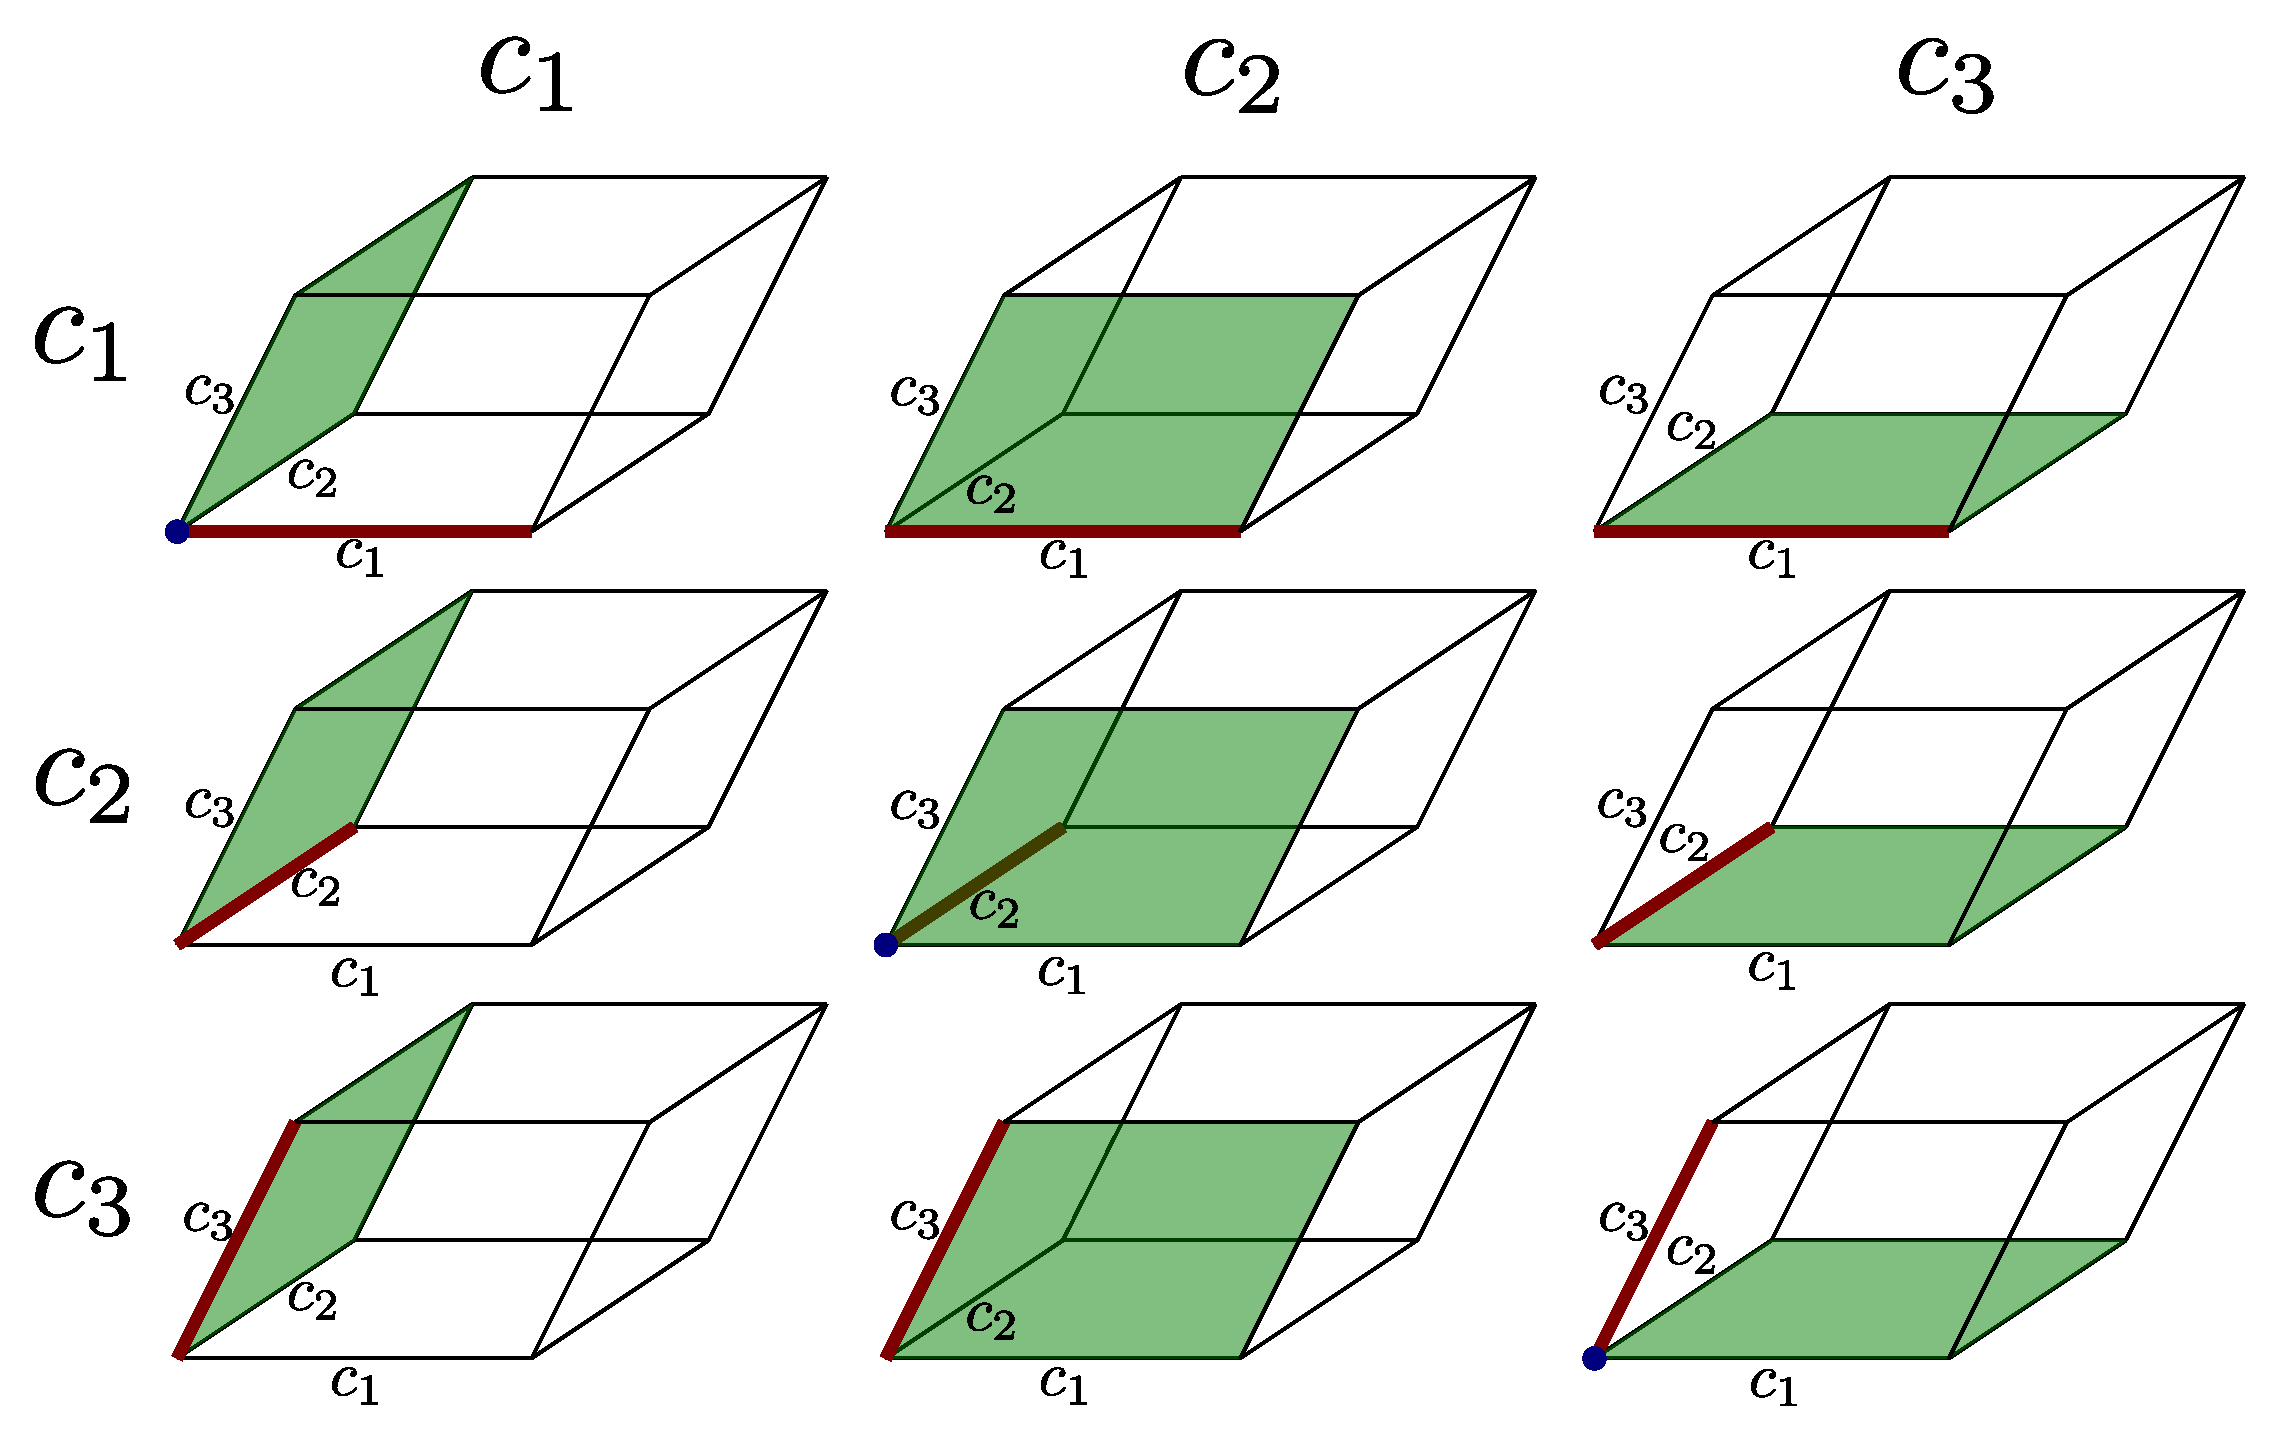
\includegraphics[width = 0.5\textwidth]{Coordinate_systems/path_surface_intersection_cell}
}
\end{tabular}

\vspace{1mm}

In summary, 
\[\alpha_{i, (k_1,k_2,k_3)} \bullet \sigma_{j, (k_1,k_2,k_3)} = \left\{\begin{array}{cc} \theta_{(k_1, k_2, k_3)} & (i = j) \\ 0 & (i \neq j) \end{array}\right.\]

The total weight of point \(\theta_{(k_1,k_2,k_3)}\) is: 
\[J_1 F_1 B_1 h_1 \Delta c_1 \Delta c_2 \Delta c_3 + J_2 F_2 B_2 h_2 \Delta c_1 \Delta c_2 \Delta c_3 + J_1 F_1 B_2 h_2 \Delta c_1 \Delta c_2 \Delta c_3 
= \left(\sum_i J_i F_i B_i h_i\right) \Delta c_1 \Delta c_2 \Delta c_3\]

The density over the current cell is the point weight divided by the volume:
\[\frac{\left(\sum_i J_i F_i B_i h_i\right) \Delta c_1 \Delta c_2 \Delta c_3}{V \Delta c_1 \Delta c_2 \Delta c_3} = \sum_i J_i F_i \frac{B_i h_i}{V}\]

The intersection is therefore:

\begin{thm}
\[\mathbf{J} \bullet \mathbf{F} = \begin{bmatrix} J_1 \\ J_2 \\ J_3 \end{bmatrix} \bullet \begin{bmatrix} F_1 \\ F_2 \\ F_3 \end{bmatrix} = \frac{B_1 h_1}{V} J_1 F_1 + \frac{B_2 h_2}{V} J_2 F_2 + \frac{B_3 h_3}{V} J_3 F_3 = \sum_i \frac{B_i h_i}{V} J_i F_i\]
\end{thm}



\subsection{Computing surface-surface intersections}

Consider the multi-surfaces \(\mathbf{F} = [i : F_i] = \begin{bmatrix} F_1 \\ F_2 \\ F_3 \end{bmatrix}\) and \(\mathbf{G} = [i : G_i] = \begin{bmatrix} G_1 \\ G_2 \\ G_3 \end{bmatrix}\). The multi-path intersection \(\mathbf{F} \times \mathbf{G}\) can be computed as follows:

For simplicity, the parameter \(\mathbf{q}\) will be hidden in the notation.

\vspace{1mm}

\begin{tabular}{cc}
\parbox{0.5\textwidth}{
Consider an arbitrary point \(\mathbf{q}\), and let \((k_1, k_2, k_3)\) index the cell at \(\mathbf{q}\). 

For each \(i = 1, 2, 3\), the weight assigned to the lattice tile \(\sigma_{i,(k_1,k_2,k_3)}\) by \(\mathbf{F}\) is the surface density \(F_i\) multiplied by the thickness of the cell to get \(F_i \cdot h_i \cdot \Delta c_i\). 

For each \(j = 1, 2, 3\), the weight assigned to the lattice tile \(\sigma_{j,(k_1,k_2,k_3)}\) by \(\mathbf{G}\) is the surface density \(G_j\) multiplied by the thickness of the cell to get \(G_j \cdot h_j \cdot \Delta c_j\). 

When \(i = j\), the lattice tiles \(\sigma_{i, (k_1, k_2, k_3)}\) and \(\sigma_{j, (k_1, k_2, k_3)}\) are parallel (as depicted on the right), and there is no intersection. 

When \(i \neq j\), the lattice tiles \(\sigma_{i, (k_1, k_2, k_3)}\) and \(\sigma_{j, (k_1, k_2, k_3)}\) intersect. 
} & \parbox{0.5\textwidth}{
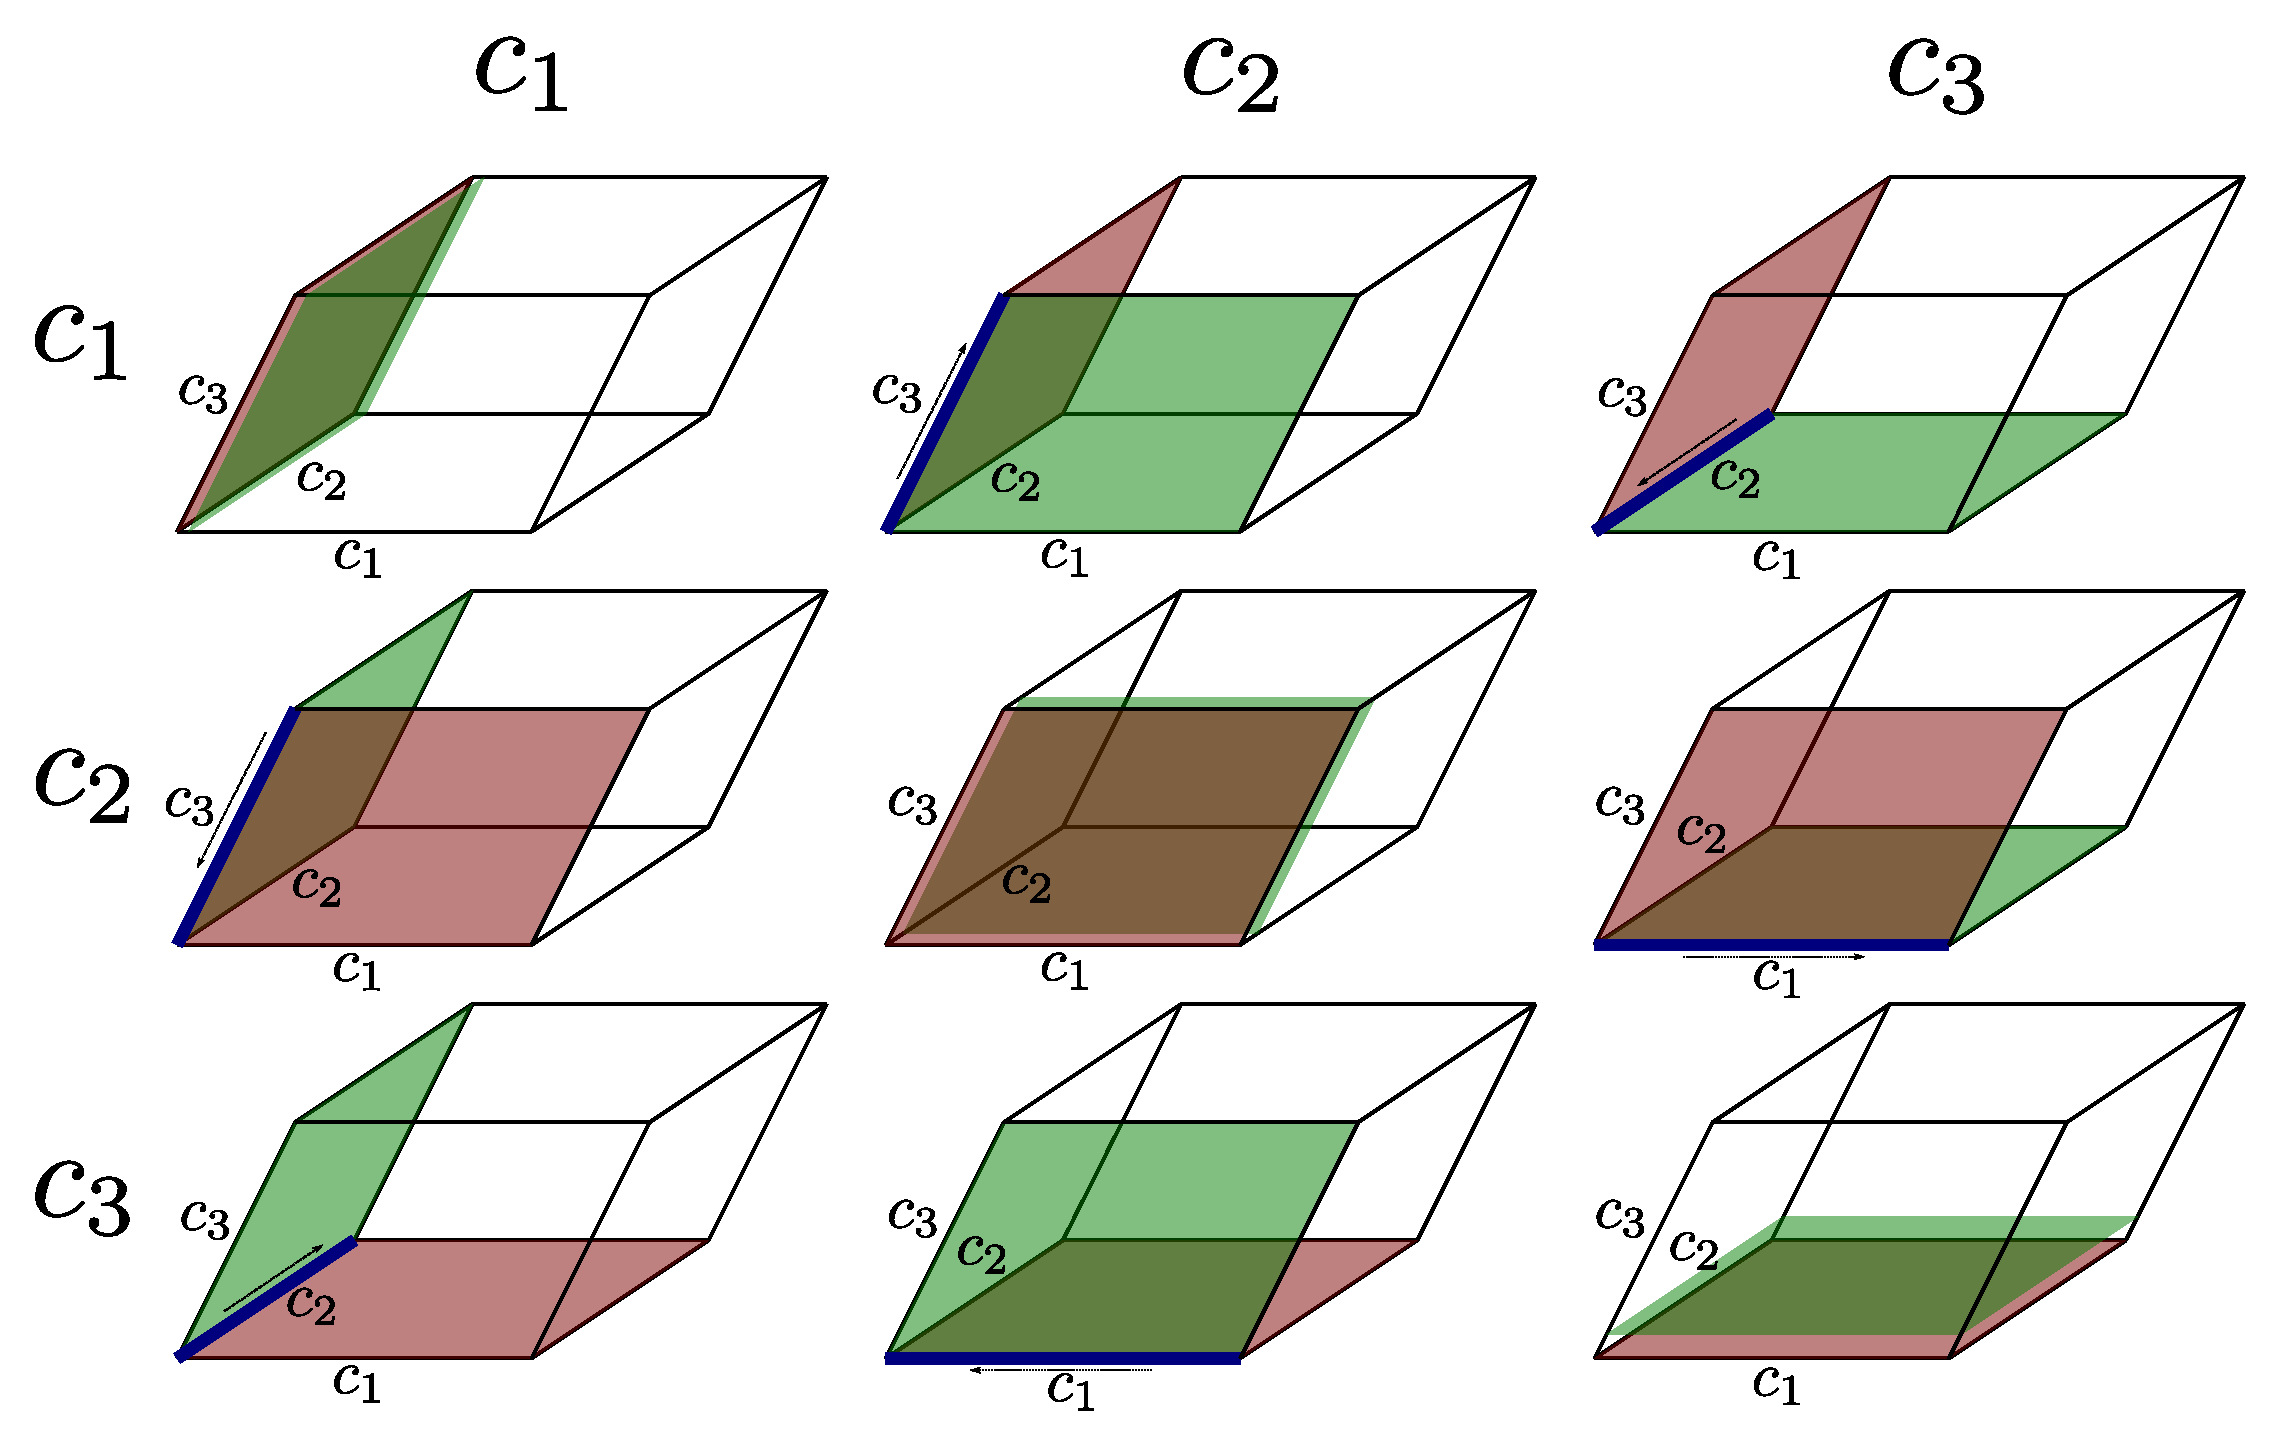
\includegraphics[width = 0.5\textwidth]{Coordinate_systems/surface_surface_intersection_cell}
}
\end{tabular}

\vspace{1mm}

When \(j = i + 1\), \(\sigma_{i, (k_1, k_2, k_3)} \times \sigma_{i+1, (k_1, k_2, k_3)} = \alpha_{i+2, (k_1, k_2, k_3)}\), as depicted on the right. 

When \(j = i + 2\), \(\sigma_{i, (k_1, k_2, k_3)} \times \sigma_{i+2, (k_1, k_2, k_3)} = -\alpha_{i+1, (k_1, k_2, k_3)}\), as depicted on the right. {\bf Note the reversed orientation.} 

In summary, 
\[\sigma_{i, (k_1,k_2,k_3)} \times \sigma_{j, (k_1,k_2,k_3)} = \left\{\begin{array}{cc} 0 & (j = i) \\ \alpha_{i+2, (k_1, k_2, k_3)} & (j = i+1) \\ -\alpha_{i+1, (k_1, k_2, k_3)} & (j = i+2) \end{array}\right.\]

Now putting everything together, for each index \(i = 1, 2, 3\), the path \(\alpha_{i, (k_1, k_2, k_3)}\) is the intersection of \(\sigma_{i+1, (k_1, k_2, k_3)}\) with \(\sigma_{i+2, (k_1, k_2, k_3)}\), as well as the reverse of the intersection of \(\sigma_{i+2, (k_1, k_2, k_3)}\) with \(\sigma_{i+1, (k_1, k_2, k_3)}\).

Since the weight of tile \(\sigma_{j, (k_1, k_2, k_3)}\) is \(F_j h_j \Delta c_j\) for \(\mathbf{F}\), and \(G_j h_j \Delta c_j\) for \(\mathbf{G}\), the total weight of path \(\alpha_{i, (k_1,k_2,k_3)}\) is: 
\begin{align*}
& (F_{i+1} h_{i+1} \Delta c_{i+1})(G_{i+2} h_{i+2} \Delta c_{i+2}) - (F_{i+2} h_{i+2} \Delta c_{i+2})(G_{i+1} h_{i+1} \Delta c_{i+1}) \\
& = F_{i+1} G_{i+2} h_{i+1} h_{i+2} \Delta c_{i+1} \Delta c_{i+2} - F_{i+2} G_{i+1} h_{i+2} h_{i+1} \Delta c_{i+2} \Delta c_{i+1} \\
& = (F_{i+1} G_{i+2} - F_{i+2} G_{i+1})h_{i+1} h_{i+2} \Delta c_{i+1} \Delta c_{i+2}
\end{align*}

The path density is the path weight divided by the cross sectional area:
\[\frac{(F_{i+1} G_{i+2} - F_{i+2} G_{i+1})h_{i+1} h_{i+2} \Delta c_{i+1} \Delta c_{i+2}}{B_i \Delta c_{i+1} \Delta c_{i+2}} = (F_{i+1} G_{i+2} - F_{i+2} G_{i+1})\frac{h_{i+1} h_{i+2}}{B_i}\]

The intersection is therefore:

\begin{thm}
\[\mathbf{F} \times \mathbf{G} = \begin{bmatrix} F_1 \\ F_2 \\ F_3 \end{bmatrix} \times \begin{bmatrix} G_1 \\ G_2 \\ G_3 \end{bmatrix}
 = \begin{bmatrix} \frac{h_2 h_3}{B_1}(F_2 G_3 - F_3 G_2) \\ \frac{h_3 h_1}{B_2}(F_3 G_1 - F_1 G_3) \\ \frac{h_1 h_2}{B_3}(F_1 G_2 - F_2 G_1) \end{bmatrix}
 = \left[i : \frac{h_{i+1} h_{i+2}}{B_i} (F_{i+1} G_{i+2} - F_{i+2} G_{i+1})\right]\]
\end{thm}



\subsection*{Summary}

\begin{itemize}
%\item Given a multi-point \(\rho\) and a multi-volume \(U\), then the intersection is the multi-point:
%
%\[\rho \cdot U = \rho(\mathbf{q}) \cdot U(\mathbf{q})\]


\item Given a multi-path \(\mathbf{J} = [i : J_i] = \begin{bmatrix} J_1 \\ J_2 \\ J_3 \end{bmatrix}\) and a multi-surface \(\mathbf{F} = [i : F_i] = \begin{bmatrix} F_1 \\ F_2 \\ F_3 \end{bmatrix}\), then the intersection is the multi-point:

\[\mathbf{J} \bullet \mathbf{F} = \begin{bmatrix} J_1 \\ J_2 \\ J_3 \end{bmatrix} \bullet \begin{bmatrix} F_1 \\ F_2 \\ F_3 \end{bmatrix} = \frac{B_1 h_1}{V} J_1 F_1 + \frac{B_2 h_2}{V} J_2 F_2 + \frac{B_3 h_3}{V} J_3 F_3 = \sum_i \frac{B_i h_i}{V} J_i F_i\]


%\item Given a multi-path \(\mathbf{J} = [i : J_i] = \begin{bmatrix} J_1 \\ J_2 \\ J_3 \end{bmatrix}\) and a multi-volume \(U\), then the intersection is the multi-path:
%
%\[\mathbf{J} \cdot U = \begin{bmatrix} J_1 \cdot U \\ J_2 \cdot U \\ J_3 \cdot U \end{bmatrix} = [i : J_i \cdot U]\]


\item Given multi-surfaces \(\mathbf{F} = [i : F_i] = \begin{bmatrix} F_1 \\ F_2 \\ F_3 \end{bmatrix}\) and \(\mathbf{G} = [i : G_i] = \begin{bmatrix} G_1 \\ G_2 \\ G_3 \end{bmatrix}\), then the intersection is the multi-path:

\[\mathbf{F} \times \mathbf{G} = \begin{bmatrix} F_1 \\ F_2 \\ F_3 \end{bmatrix} \times \begin{bmatrix} G_1 \\ G_2 \\ G_3 \end{bmatrix}
 = \begin{bmatrix} \frac{h_2 h_3}{B_1}(F_2 G_3 - F_3 G_2) \\ \frac{h_3 h_1}{B_2}(F_3 G_1 - F_1 G_3) \\ \frac{h_1 h_2}{B_3}(F_1 G_2 - F_2 G_1) \end{bmatrix}
 = \left[i : \frac{h_{i+1} h_{i+2}}{B_i} (F_{i+1} G_{i+2} - F_{i+2} G_{i+1})\right]\]



%\item Given a multi-surface \(\mathbf{F} = [i : F_i] = \begin{bmatrix} F_1 \\ F_2 \\ F_3 \end{bmatrix}\) and a multi-volume \(U\), then the intersection is the multi-surface:
%
%\[\mathbf{F} \cdot U = \begin{bmatrix} F_1 \cdot U \\ F_2 \cdot U \\ F_3 \cdot U \end{bmatrix} = [i : F_i \cdot U]\]
%
%
%
%\item Given multi-volumes \(U\) and \(T\), then the intersection is the multi-volume:
%
%\[U \cdot T = U(\mathbf{q}) \cdot T(\mathbf{q})\]
\end{itemize}





\section{Computing boundaries}

Given a function \(f(c_1, c_2, c_3)\), the notation \(\frac{\partial}{\partial c_1}(f(c_1, c_2, c_3))\) will denote the rate of change of the quantity \(f(c_1, c_2, c_3)\) with respect to \(c_1\). Similar notation exists for \(c_2\) and \(c_3\), respectively \(\frac{\partial}{\partial c_2}(f(c_1, c_2, c_3))\) and \(\frac{\partial}{\partial c_3}(f(c_1, c_2, c_3))\).

More specifically, 
\[\frac{\partial}{\partial c_1}(f(c_1, c_2, c_3)) = \frac{f(c_1, c_2, c_3) - f(c_1 - \Delta c_1, c_2, c_3)}{\Delta c_1}\]
is the change in \(f(c_1, c_2, c_3)\) between {\bf adjacent cells} in principal direction \(1\) divided by the change in \(c_1\).
\[\frac{\partial}{\partial c_2}(f(c_1, c_2, c_3)) = \frac{f(c_1, c_2, c_3) - f(c_1, c_2 - \Delta c_2, c_3)}{\Delta c_2}\]
is the change in \(f(c_1, c_2, c_3)\) between {\bf adjacent cells} in principal direction \(2\) divided by the change in \(c_2\).
\[\frac{\partial}{\partial c_3}(f(c_1, c_2, c_3)) = \frac{f(c_1, c_2, c_3) - f(c_1, c_2, c_3 - \Delta c_3)}{\Delta c_3}\]
is the change in \(f(c_1, c_2, c_3)\) between {\bf adjacent cells} in principal direction \(3\) divided by the change in \(c_3\).




\subsection{Computing path endpoints}

Consider the multi-path \(\mathbf{J} = [i : J_i] = \begin{bmatrix} J_1 \\ J_2 \\ J_3 \end{bmatrix}\). The multi-point end points \(\nabla \bullet \mathbf{J}\) can be computed as follows:

Let \((c_1, c_2, c_3)\) denote an arbitrary position, and let \((k_1, k_2, k_3)\) index the cell that contains \((c_1, c_2, c_3)\). The lattice line segments \(\alpha_{1,(k_1,k_2,k_3)}\), \(\alpha_{1,(k_1-1,k_2,k_3)}\), \(\alpha_{2,(k_1,k_2,k_3)}\), \(\alpha_{2,(k_1,k_2-1,k_3)}\), \(\alpha_{3,(k_1,k_2,k_3)}\), and \(\alpha_{3,(k_1,k_2,k_3-1)}\) have endpoints at \(\theta_{(k_1, k_2, k_3)}\). 

The weights of these paths are:
\begin{itemize}
\item The weight of \(\alpha_{1,(k_1,k_2,k_3)}\) is \(J_1(c_1,c_2,c_3) B_1(c_1, c_2, c_3) \Delta c_2 \Delta c_3\)
\item The weight of \(\alpha_{1,(k_1-1,k_2,k_3)}\) is \(J_1(c_1 - \Delta c_1,c_2,c_3) B_1(c_1 - \Delta c_1, c_2, c_3) \Delta c_2 \Delta c_3\)
\item The weight of \(\alpha_{2,(k_1,k_2,k_3)}\) is \(J_2(c_1,c_2,c_3) B_2(c_1, c_2, c_3) \Delta c_3 \Delta c_1\)
\item The weight of \(\alpha_{2,(k_1,k_2-1,k_3)}\) is \(J_2(c_1,c_2 - \Delta c_2,c_3) B_2(c_1, c_2 - \Delta c_2, c_3) \Delta c_3 \Delta c_1\)
\item The weight of \(\alpha_{3,(k_1,k_2,k_3)}\) is \(J_3(c_1,c_2,c_3) B_3(c_1, c_2, c_3) \Delta c_1 \Delta c_2\)
\item The weight of \(\alpha_{3,(k_1,k_2,k_3-1)}\) is \(J_3(c_1,c_2,c_3 - \Delta c_3) B_3(c_1, c_2, c_3 - \Delta c_3) \Delta c_1 \Delta c_2\)
\end{itemize}

The total endpoint weight at \(\theta_{(k_1, k_2, k_3)}\) is 
\begin{align*}
& J_1(c_1,c_2,c_3) B_1(c_1, c_2, c_3) \Delta c_2 \Delta c_3 - J_1(c_1 - \Delta c_1,c_2,c_3) B_1(c_1 - \Delta c_1, c_2, c_3) \Delta c_2 \Delta c_3 \\ 
& + J_2(c_1,c_2,c_3) B_2(c_1, c_2, c_3) \Delta c_3 \Delta c_1 - J_2(c_1,c_2 - \Delta c_2,c_3) B_2(c_1, c_2 - \Delta c_2, c_3) \Delta c_3 \Delta c_1 \\
& + J_3(c_1,c_2,c_3) B_3(c_1, c_2, c_3) \Delta c_1 \Delta c_2 - J_3(c_1,c_2,c_3 - \Delta c_3) B_3(c_1, c_2, c_3 - \Delta c_3) \Delta c_1 \Delta c_2 \\
= & (J_1(c_1,c_2,c_3) B_1(c_1, c_2, c_3) - J_1(c_1 - \Delta c_1,c_2,c_3) B_1(c_1 - \Delta c_1, c_2, c_3)) \Delta c_2 \Delta c_3 \\ 
& + (J_2(c_1,c_2,c_3) B_2(c_1, c_2, c_3) - J_2(c_1,c_2 - \Delta c_2,c_3) B_2(c_1, c_2 - \Delta c_2, c_3)) \Delta c_3 \Delta c_1 \\ 
& + (J_3(c_1,c_2,c_3) B_3(c_1, c_2, c_3) - J_3(c_1,c_2,c_3 - \Delta c_3) B_3(c_1, c_2, c_3 - \Delta c_3)) \Delta c_1 \Delta c_2  
\end{align*}

\begin{tabular}{cc}
\parbox{0.4\textwidth}{
On the right is shown how the endpoint weights of the line segment pairs \(\alpha_{1,(k_1,k_2,k_3)}\) and \(\alpha_{1,(k_1-1,k_2,k_3)}\); \(\alpha_{2,(k_1,k_2,k_3)}\) and \(\alpha_{2,(k_1,k_2-1,k_3)}\); and \(\alpha_{3,(k_1,k_2,k_3)}\) and \(\alpha_{3,(k_1,k_2,k_3-1)}\) partially cancel out at the vertex \(\theta_{(k_1,k_2,k_3)}\).
} & \parbox{0.6\textwidth}{
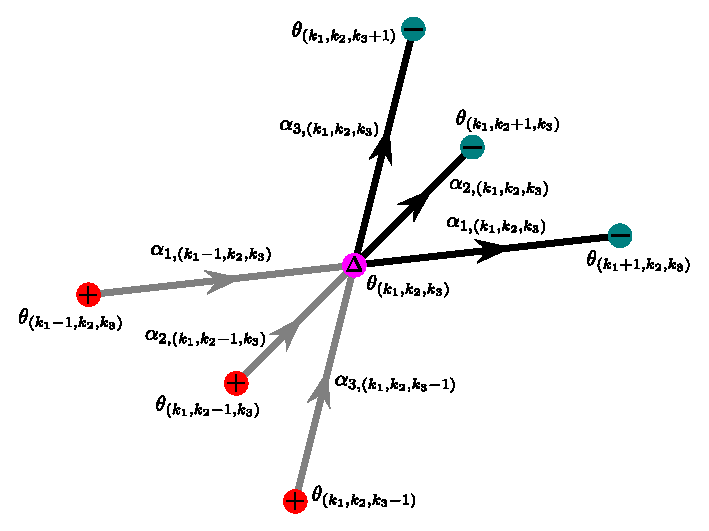
\includegraphics[width = 0.6\textwidth]{Coordinate_systems/path_endpoint_cell}
}
\end{tabular}

Spreading the weight of \(\theta_{(k_1, k_2, k_3)}\) over the volume of cell \((k_1, k_2, k_3)\) gives:

\begin{align*}
\nabla \bullet \mathbf{J} = & \frac{1}{V \Delta c_1 \Delta c_2 \Delta c_3}\bigg((J_1(c_1,c_2,c_3) B_1(c_1, c_2, c_3) - J_1(c_1 - \Delta c_1,c_2,c_3) B_1(c_1 - \Delta c_1, c_2, c_3))\Delta c_2 \Delta c_3 \\
& \quad\quad\quad\quad\quad + (J_2(c_1,c_2,c_3) B_2(c_1, c_2, c_3) - J_2(c_1,c_2 - \Delta c_2,c_3) B_2(c_1, c_2 - \Delta c_2, c_3)) \Delta c_3 \Delta c_1 \\ 
& \quad\quad\quad\quad\quad + (J_3(c_1,c_2,c_3) B_3(c_1, c_2, c_3) - J_3(c_1,c_2,c_3 - \Delta c_3) B_3(c_1, c_2, c_3 - \Delta c_3)) \Delta c_1 \Delta c_2 \bigg) \\
= & \frac{1}{V}\bigg(\frac{J_1(c_1,c_2,c_3) B_1(c_1, c_2, c_3) - J_1(c_1 - \Delta c_1,c_2,c_3) B_1(c_1 - \Delta c_1, c_2, c_3)}{\Delta c_1} \\
& \quad\quad + \frac{J_2(c_1,c_2,c_3) B_2(c_1, c_2, c_3) - J_2(c_1,c_2 - \Delta c_2,c_3) B_2(c_1, c_2 - \Delta c_2, c_3)}{\Delta c_2} \\ 
& \quad\quad + \frac{J_3(c_1,c_2,c_3) B_3(c_1, c_2, c_3) - J_3(c_1,c_2,c_3 - \Delta c_3) B_3(c_1, c_2, c_3 - \Delta c_3)}{\Delta c_3}\bigg) \\
= & \frac{1}{V}\left(\frac{\partial}{\partial c_1}(J_1 B_1) + \frac{\partial}{\partial c_2}(J_2 B_2) + \frac{\partial}{\partial c_3}(J_3 B_3)\right)
\end{align*}

Therefore:
\begin{thm}
The endpoints of multi-path \(\mathbf{J} = [i : J_i] = \begin{bmatrix} J_1 \\ J_2 \\ J_3 \end{bmatrix}\) is the multi-point:

\[\nabla \bullet \mathbf{J} = \nabla \bullet \begin{bmatrix} J_1 \\ J_2 \\ J_3 \end{bmatrix} = \frac{1}{V}\left(\frac{\partial}{\partial c_1}(B_1 J_1) + \frac{\partial}{\partial c_2}(B_2 J_2) + \frac{\partial}{\partial c_3}(B_3 J_3)\right) = \frac{1}{V}\sum_i \frac{\partial}{\partial c_i} (B_i J_i)\]
\end{thm}



\subsection{Computing surface boundaries}

Consider the multi-surface \(\mathbf{F} = [i : F_i] = \begin{bmatrix} F_1 \\ F_2 \\ F_3 \end{bmatrix}\). The multi-path boundary \(\nabla \times \mathbf{F}\) can be computed as follows:

Let \((c_1, c_2, c_3)\) denote an arbitrary position, and let \((k_1, k_2, k_3)\) index the cell that contains \((c_1, c_2, c_3)\). For notational simplicity, the weight that the counter-clockwise boundary assigns to the lattice line segment \(\alpha_{1, (k_1, k_2, k_3)}\) will be computed. The weights assigned to \(\alpha_{2, (k_1, k_2, k_3)}\) and \(\alpha_{3, (k_1, k_2, k_3)}\) can be computed in an exactly analogous manner. 

\begin{tabular}{cc}
\parbox{0.5\textwidth}{
The lattice tiles \(\sigma_{3, (k_1, k_2, k_3)}\); \(\sigma_{3, (k_1, k_2-1, k_3)}\); \(\sigma_{2, (k_1, k_2, k_3)}\); and \(\sigma_{2, (k_1, k_2, k_3-1)}\) have the lattice line segment \(\alpha_{1, (k_1, k_2, k_3)}\) as part of their boundary, as depicted on the right. The weights of these tiles are respectively 
\begin{itemize}
\item \(F_3(c_1,c_2,c_3)h_3(c_1,c_2,c_3)\Delta c_3\) 
\item \(F_3(c_1,c_2 - \Delta c_2,c_3)h_3(c_1,c_2 - \Delta c_2,c_3)\Delta c_3\) 
\item \(F_2(c_1,c_2,c_3)h_2(c_1,c_2,c_3)\Delta c_2\)
\item \(F_2(c_1,c_2,c_3 - \Delta c_3)h_2(c_1,c_2,c_3 - \Delta c_3)\Delta c_2\)   
\end{itemize}    
From the image of the right, the counterclockwise boundaries of these tiles add to the weight of \(\alpha_{1, (k_1, k_2, k_3)}\) in the case of \(\sigma_{3, (k_1, k_2, k_3)}\) and \(\sigma_{2, (k_1, k_2, k_3-1)}\), and subtract from the weight of \(\alpha_{1, (k_1, k_2, k_3)}\) in the case of \(\sigma_{3, (k_1, k_2-1, k_3)}\) and \(\sigma_{2, (k_1, k_2, k_3)}\)
} & \parbox{0.5\textwidth}{
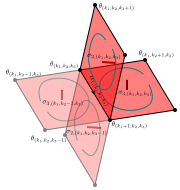
\includegraphics[width = 0.5\textwidth]{Coordinate_systems/surface_boundary_cell}
}
\end{tabular}

The total weight of \(\alpha_{1, (k_1, k_2, k_3)}\) is:
\begin{align*}
& F_3(c_1,c_2,c_3)h_3(c_1,c_2,c_3)\Delta c_3 
- F_3(c_1,c_2 - \Delta c_2,c_3)h_3(c_1,c_2 - \Delta c_2,c_3)\Delta c_3 \\
& - F_2(c_1,c_2,c_3)h_2(c_1,c_2,c_3)\Delta c_2
+ F_2(c_1,c_2,c_3 - \Delta c_3)h_2(c_1,c_2,c_3 - \Delta c_3)\Delta c_2 \\ 
= & (F_3(c_1,c_2,c_3)h_3(c_1,c_2,c_3) 
- F_3(c_1,c_2 - \Delta c_2,c_3)h_3(c_1,c_2 - \Delta c_2,c_3))\Delta c_3 \\
& - (F_2(c_1,c_2,c_3)h_2(c_1,c_2,c_3)
- F_2(c_1,c_2,c_3 - \Delta c_3)h_2(c_1,c_2,c_3 - \Delta c_3))\Delta c_2
\end{align*}

Spreading the weight of \(\alpha_{1, (k_1, k_2, k_3)}\) over the cross sectional area of cell \((k_1, k_2, k_3)\) gives:
\begin{align*}
& \frac{1}{B_1 \Delta c_2 \Delta c_3}\bigg((F_3(c_1,c_2,c_3)h_3(c_1,c_2,c_3) 
- F_3(c_1,c_2 - \Delta c_2,c_3)h_3(c_1,c_2 - \Delta c_2,c_3))\Delta c_3 \\ 
& \quad\quad\quad - (F_2(c_1,c_2,c_3)h_2(c_1,c_2,c_3)
- F_2(c_1,c_2,c_3 - \Delta c_3)h_2(c_1,c_2,c_3 - \Delta c_3))\Delta c_2\bigg) \\
= & \frac{1}{B_1}\bigg(\frac{F_3(c_1,c_2,c_3)h_3(c_1,c_2,c_3) - F_3(c_1,c_2 - \Delta c_2,c_3)h_3(c_1,c_2 - \Delta c_2,c_3)}{\Delta c_2} \\ 
& \quad\quad\quad - \frac{F_2(c_1,c_2,c_3)h_2(c_1,c_2,c_3)
- F_2(c_1,c_2,c_3 - \Delta c_3)h_2(c_1,c_2,c_3 - \Delta c_3)}{\Delta c_3}\bigg) \\
= & \frac{1}{B_1}\left(\frac{\partial}{\partial c_2}(F_3 h_3) - \frac{\partial}{\partial c_3}(F_2 h_2)\right)
\end{align*}

Performing analogous calculations for \(\alpha_{2, (k_1, k_2, k_3)}\) and \(\alpha_{3, (k_1, k_2, k_3)}\) yields the general expression for the path weight density at \(\alpha_{i, (k_1, k_2, k_3)}\):
\[\frac{1}{B_i}\left(\frac{\partial}{\partial c_{i+1}}(F_{i+2} h_{i+2}) - \frac{\partial}{\partial c_{i+2}}(F_{i+1} h_{i+1})\right)\]

Therefore:
\begin{thm}
The counterclockwise boundary of multi-surface \(\mathbf{F} = [i : F_i] = \begin{bmatrix} F_1 \\ F_2 \\ F_3 \end{bmatrix}\) is the multi-path:

\[\nabla \times \mathbf{F} = \nabla \times \begin{bmatrix} F_1 \\ F_2 \\ F_3 \end{bmatrix} = \begin{bmatrix} \frac{1}{B_1}\left(\frac{\partial}{\partial c_2}(h_3 F_3) - \frac{\partial}{\partial c_3}(h_2 F_2)\right) \\ \frac{1}{B_2}\left(\frac{\partial}{\partial c_3}(h_1 F_1) - \frac{\partial}{\partial c_1}(h_3 F_3)\right) \\ \frac{1}{B_3}\left(\frac{\partial}{\partial c_1}(h_2 F_2) - \frac{\partial}{\partial c_2}(h_1 F_1)\right) \end{bmatrix} = \left[ i : \frac{1}{B_i}\left(\frac{\partial}{\partial c_{i+1}}(h_{i+2} F_{i+2}) - \frac{\partial}{\partial c_{i+2}}(h_{i+1} F_{i+1})\right) \right]\]
\end{thm}




\subsection{Computing volume surfaces}

Consider the multi-volume \(U\). The multi-surface inwards oriented surface \(\nabla U\) can be computed as follows:

Let \((c_1, c_2, c_3)\) denote an arbitrary position, and let \((k_1, k_2, k_3)\) index the cell that contains \((c_1, c_2, c_3)\). For notational simplicity, the weight that the inwards-oriented surface assigns to the lattice tile \(\sigma_{1, (k_1, k_2, k_3)}\) will be computed. The weights assigned to \(\sigma_{2, (k_1, k_2, k_3)}\) and \(\sigma_{3, (k_1, k_2, k_3)}\) can be computed in an exactly analogous manner. 

The cell volumes \(\Omega_{(k_1, k_2, k_3)}\) and \(\Omega_{(k_1-1,k_2,k_3)}\) have the lattice tile \(\sigma_{1,(k_1,k_2,k_3)}\) as part of their boundary, as depicted below. 

\begin{center}
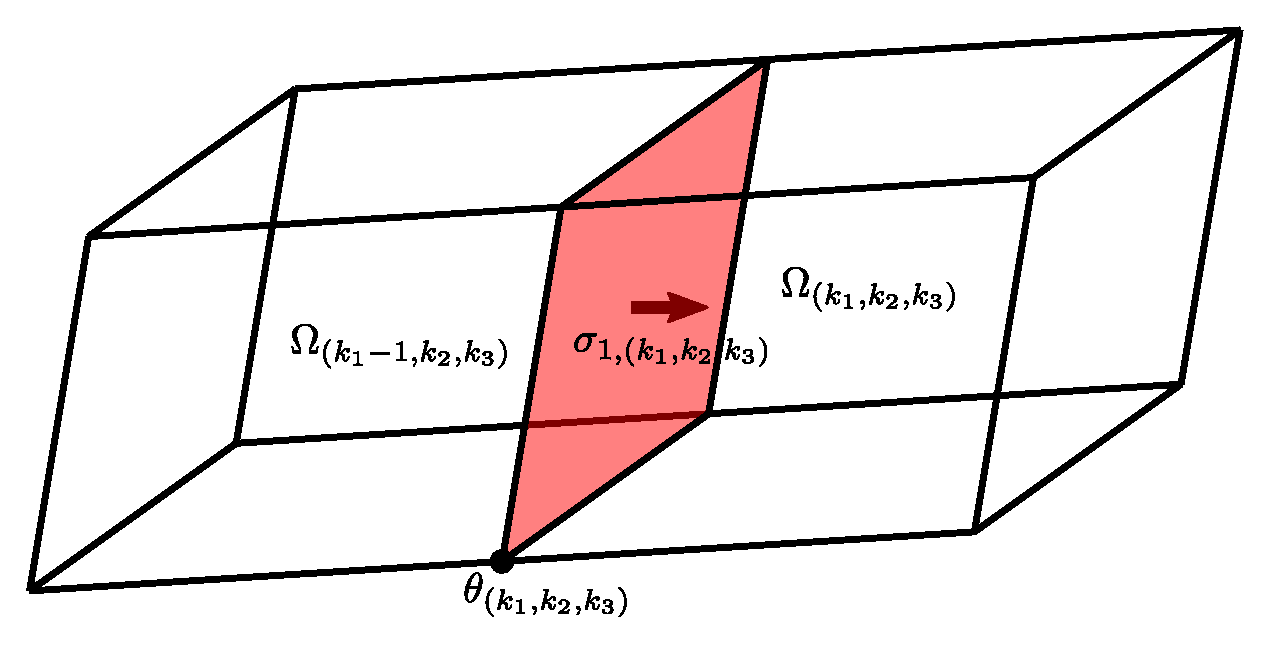
\includegraphics[width = 0.6\textwidth]{Coordinate_systems/volume_surface_cell}
\end{center}

The weights of these volumes are respectively \(U(c_1, c_2, c_3)\) and \(U(c_1 - \Delta c_1, c_2, c_3)\). The total weight of \(\sigma_{1,(k_1,k_2,k_3)}\) is:
\[U(c_1,c_2,c_3) - U(c_1 - \Delta c_1, c_2, c_3)\]

Spreading the weight of \(\sigma_{1, (k_1,k_2,k_3)}\) over the thickness of cell \((k_1, k_2, k_3)\) gives:
\begin{align*}
& \frac{1}{h_1 \Delta c_1}(U(c_1,c_2,c_3) - U(c_1 - \Delta c_1, c_2, c_3)) 
= \frac{1}{h_1}\frac{U(c_1,c_2,c_3) - U(c_1 - \Delta c_1, c_2, c_3)}{\Delta c_1} 
= \frac{1}{h_1}\frac{\partial}{\partial c_1}(U)
\end{align*}

Performing analogous calculations for \(\sigma_{2, (k_1, k_2, k_3)}\) and \(\sigma_{3, (k_1, k_2, k_3)}\) yields the general expression for the surface weight density at \(\sigma_{i, (k_1, k_2, k_3)}\):
\[\frac{1}{h_i}\frac{\partial}{\partial c_i}(U)\]

Therefore:
\begin{thm}
The inwards oriented surface of multi-volume \(U\) is the multi-surface:

\[\nabla U = \begin{bmatrix} \frac{1}{h_1}\frac{\partial}{\partial c_1}(U) \\ \frac{1}{h_2}\frac{\partial}{\partial c_2}(U) \\ \frac{1}{h_3}\frac{\partial}{\partial c_3}(U) \end{bmatrix} = \left[ i :  \frac{1}{h_i}\frac{\partial}{\partial c_i}(U)\right]\]
\end{thm}



\subsection*{Summary}

\begin{itemize}
\item The endpoints of multi-path \(\mathbf{J} = [i : J_i] = \begin{bmatrix} J_1 \\ J_2 \\ J_3 \end{bmatrix}\) is the multi-point:

\[\nabla \bullet \mathbf{J} = \nabla \bullet \begin{bmatrix} J_1 \\ J_2 \\ J_3 \end{bmatrix} = \frac{1}{V}\left(\frac{\partial}{\partial c_1}(B_1 J_1) + \frac{\partial}{\partial c_2}(B_2 J_2) + \frac{\partial}{\partial c_3}(B_3 J_3)\right) = \frac{1}{V}\sum_i \frac{\partial}{\partial c_i} (B_i J_i)\]

%%%%%%%%%%%%%%%%%%%%%%%%%

\item The counterclockwise boundary of multi-surface \(\mathbf{F} = [i : F_i] = \begin{bmatrix} F_1 \\ F_2 \\ F_3 \end{bmatrix}\) is the multi-path:

\[\nabla \times \mathbf{F} = \nabla \times \begin{bmatrix} F_1 \\ F_2 \\ F_3 \end{bmatrix} = \begin{bmatrix} \frac{1}{B_1}\left(\frac{\partial}{\partial c_2}(h_3 F_3) - \frac{\partial}{\partial c_3}(h_2 F_2)\right) \\ \frac{1}{B_2}\left(\frac{\partial}{\partial c_3}(h_1 F_1) - \frac{\partial}{\partial c_1}(h_3 F_3)\right) \\ \frac{1}{B_3}\left(\frac{\partial}{\partial c_1}(h_2 F_2) - \frac{\partial}{\partial c_2}(h_1 F_1)\right) \end{bmatrix} = \left[ i : \frac{1}{B_i}\left(\frac{\partial}{\partial c_{i+1}}(h_{i+2} F_{i+2}) - \frac{\partial}{\partial c_{i+2}}(h_{i+1} F_{i+1})\right) \right]\]

%%%%%%%%%%%%%%%%%%%%%%%%%

\item The inwards oriented surface of multi-volume \(U\) is the multi-surface:

\[\nabla U = \begin{bmatrix} \frac{1}{h_1}\frac{\partial}{\partial c_1}(U) \\ \frac{1}{h_2}\frac{\partial}{\partial c_2}(U) \\ \frac{1}{h_3}\frac{\partial}{\partial c_3}(U) \end{bmatrix} = \left[ i :  \frac{1}{h_i}\frac{\partial}{\partial c_i}(U)\right]\]
\end{itemize}




\section{Select Coordinate systems}

The coordinate systems that will be considered are all {\bf orthogonal}. This means that:
\begin{itemize}
\item The parallelepipeds are rectangular prisms: the principal directions are all mutually orthogonal. 
\item For each \(i = 1, 2, 3\), the principal direction \(i\) is equivalent to the co-principal direction \(i\). 
\item For each \(i = 1, 2, 3\), 
\[h_i = l_i\]
\item For each \(i = 1, 2, 3\),
\[B_i = A_i = l_{i+1} l_{i+2}\]
\item 
\[V = l_1 l_2 l_3\]
\end{itemize}
Only the quantities \(l_1\), \(l_2\), and \(l_3\) need to be known.

The formulas for computing intersections and boundaries can be simplified in the case of orthogonal coordinate systems:

\begin{itemize}
\item Given a multi-path \(\mathbf{J} = [i : J_i] = \begin{bmatrix} J_1 \\ J_2 \\ J_3 \end{bmatrix}\) and a multi-surface \(\mathbf{F} = [i : F_i] = \begin{bmatrix} F_1 \\ F_2 \\ F_3 \end{bmatrix}\), then the intersection is the multi-point:

\[\mathbf{J} \bullet \mathbf{F} = \begin{bmatrix} J_1 \\ J_2 \\ J_3 \end{bmatrix} \bullet \begin{bmatrix} F_1 \\ F_2 \\ F_3 \end{bmatrix} = \frac{B_1 h_1}{V} J_1 F_1 + \frac{B_2 h_2}{V} J_2 F_2 + \frac{B_3 h_3}{V} J_3 F_3 = \sum_i \frac{B_i h_i}{V} J_i F_i\]

in the case of orthogonality,

\[\mathbf{J} \bullet \mathbf{F} = \begin{bmatrix} J_1 \\ J_2 \\ J_3 \end{bmatrix} \bullet \begin{bmatrix} F_1 \\ F_2 \\ F_3 \end{bmatrix} = J_1 F_1 + J_2 F_2 + J_3 F_3 = \sum_i J_i F_i\]

%%%%%%%%%%%%%%%%%%%%%%%%%

\item Given multi-surfaces \(\mathbf{F} = [i : F_i] = \begin{bmatrix} F_1 \\ F_2 \\ F_3 \end{bmatrix}\) and \(\mathbf{G} = [i : G_i] = \begin{bmatrix} G_1 \\ G_2 \\ G_3 \end{bmatrix}\), then the intersection is the multi-path:

\[\mathbf{F} \times \mathbf{G} = \begin{bmatrix} F_1 \\ F_2 \\ F_3 \end{bmatrix} \times \begin{bmatrix} G_1 \\ G_2 \\ G_3 \end{bmatrix}
 = \begin{bmatrix} \frac{h_2 h_3}{B_1}(F_2 G_3 - F_3 G_2) \\ \frac{h_3 h_1}{B_2}(F_3 G_1 - F_1 G_3) \\ \frac{h_1 h_2}{B_3}(F_1 G_2 - F_2 G_1) \end{bmatrix}
 = \left[i : \frac{h_{i+1} h_{i+2}}{B_i} (F_{i+1} G_{i+2} - F_{i+2} G_{i+1})\right]\]

in the case of orthogonality,

\[\mathbf{F} \times \mathbf{G} = \begin{bmatrix} F_1 \\ F_2 \\ F_3 \end{bmatrix} \times \begin{bmatrix} G_1 \\ G_2 \\ G_3 \end{bmatrix}
 = \begin{bmatrix} F_2 G_3 - F_3 G_2 \\ F_3 G_1 - F_1 G_3 \\ F_1 G_2 - F_2 G_1 \end{bmatrix}
 = \left[i : F_{i+1} G_{i+2} - F_{i+2} G_{i+1}\right]\]

%%%%%%%%%%%%%%%%%%%%%%%%%

\item The endpoints of multi-path \(\mathbf{J} = [i : J_i] = \begin{bmatrix} J_1 \\ J_2 \\ J_3 \end{bmatrix}\) is the multi-point:

\[\nabla \bullet \mathbf{J} = \nabla \bullet \begin{bmatrix} J_1 \\ J_2 \\ J_3 \end{bmatrix} = \frac{1}{V}\left(\frac{\partial}{\partial c_1}(B_1 J_1) + \frac{\partial}{\partial c_2}(B_2 J_2) + \frac{\partial}{\partial c_3}(B_3 J_3)\right) = \frac{1}{V}\sum_i \frac{\partial}{\partial c_i} (B_i J_i)\]

in the case of orthogonality, 

\[\nabla \bullet \mathbf{J} = \nabla \bullet \begin{bmatrix} J_1 \\ J_2 \\ J_3 \end{bmatrix} = \frac{1}{l_1 l_2 l_3}\left(\frac{\partial}{\partial c_1}(l_2 l_3 J_1) + \frac{\partial}{\partial c_2}(l_3 l_1 J_2) + \frac{\partial}{\partial c_3}(l_1 l_2 J_3)\right) = \frac{1}{l_1 l_2 l_3}\sum_i \frac{\partial}{\partial c_i} (l_{i+1} l_{i+2} J_i)\]

%%%%%%%%%%%%%%%%%%%%%%%%%

\item The counterclockwise boundary of multi-surface \(\mathbf{F} = [i : F_i] = \begin{bmatrix} F_1 \\ F_2 \\ F_3 \end{bmatrix}\) is the multi-path:

\[\nabla \times \mathbf{F} = \nabla \times \begin{bmatrix} F_1 \\ F_2 \\ F_3 \end{bmatrix} = \begin{bmatrix} \frac{1}{B_1}\left(\frac{\partial}{\partial c_2}(h_3 F_3) - \frac{\partial}{\partial c_3}(h_2 F_2)\right) \\ \frac{1}{B_2}\left(\frac{\partial}{\partial c_3}(h_1 F_1) - \frac{\partial}{\partial c_1}(h_3 F_3)\right) \\ \frac{1}{B_3}\left(\frac{\partial}{\partial c_1}(h_2 F_2) - \frac{\partial}{\partial c_2}(h_1 F_1)\right) \end{bmatrix} = \left[ i : \frac{1}{B_i}\left(\frac{\partial}{\partial c_{i+1}}(h_{i+2} F_{i+2}) - \frac{\partial}{\partial c_{i+2}}(h_{i+1} F_{i+1})\right) \right]\]

in the case of orthogonality, 

\[\nabla \times \mathbf{F} = \nabla \times \begin{bmatrix} F_1 \\ F_2 \\ F_3 \end{bmatrix} = \begin{bmatrix} \frac{1}{l_2 l_3}\left(\frac{\partial}{\partial c_2}(l_3 F_3) - \frac{\partial}{\partial c_3}(l_2 F_2)\right) \\ \frac{1}{l_3 l_1}\left(\frac{\partial}{\partial c_3}(l_1 F_1) - \frac{\partial}{\partial c_1}(l_3 F_3)\right) \\ \frac{1}{l_1 l_2}\left(\frac{\partial}{\partial c_1}(l_2 F_2) - \frac{\partial}{\partial c_2}(l_1 F_1)\right) \end{bmatrix} = \left[ i : \frac{1}{l_{i+1} l_{i+2}}\left(\frac{\partial}{\partial c_{i+1}}(l_{i+2} F_{i+2}) - \frac{\partial}{\partial c_{i+2}}(l_{i+1} F_{i+1})\right) \right]\]

%%%%%%%%%%%%%%%%%%%%%%%%%

\item The inwards oriented surface of multi-volume \(U\) is the multi-surface:

\[\nabla U = \begin{bmatrix} \frac{1}{h_1}\frac{\partial}{\partial c_1}(U) \\ \frac{1}{h_2}\frac{\partial}{\partial c_2}(U) \\ \frac{1}{h_3}\frac{\partial}{\partial c_3}(U) \end{bmatrix} = \left[ i :  \frac{1}{h_i}\frac{\partial}{\partial c_i}(U)\right]\]

in the case of orthogonality, 

\[\nabla U = \begin{bmatrix} \frac{1}{l_1}\frac{\partial}{\partial c_1}(U) \\ \frac{1}{l_2}\frac{\partial}{\partial c_2}(U) \\ \frac{1}{l_3}\frac{\partial}{\partial c_3}(U) \end{bmatrix} = \left[ i :  \frac{1}{l_i}\frac{\partial}{\partial c_i}(U)\right]\]

\end{itemize} 




\subsection{Cartesian coordinates} 

\begin{tabular}{cc}
\parbox{0.5\textwidth}{
The 3 coordinates used in {\bf Cartesian coordinates} are \(c_1 = x\), \(c_2 = y\), and \(c_3 = z\). Coordinate \(x\) is the displacement parallel to the \(x\) axis. Coordinate \(y\) is the displacement parallel to the \(y\) axis. Coordinate \(z\) is the displacement parallel to the \(z\) axis.

If \((x,y,z)\) are the coordinates of a lattice vertex, then the dimensions of the cell prism at \((x,y,z)\) are respectively:
\(1 \cdot \Delta x\); \(1 \cdot \Delta y\); and \(1 \cdot \Delta z\)

From these dimensions, the following can be derived:
} & \parbox{0.5\textwidth}{
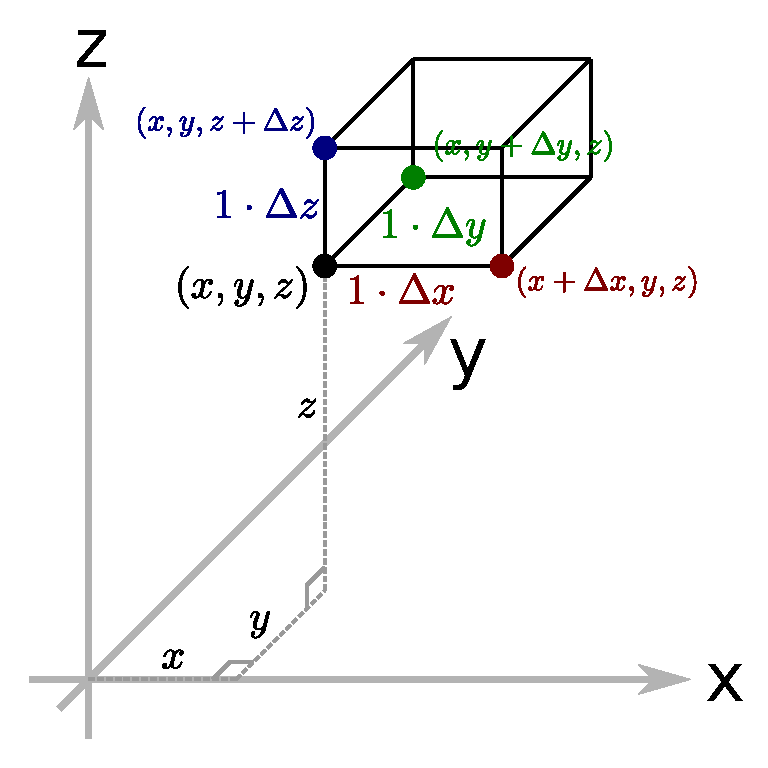
\includegraphics[width = 0.5\textwidth]{Coordinate_systems/Cartesian_coordinates}
}
\end{tabular}

\begin{itemize}
\item Given a multi-path \(\mathbf{J} = \begin{bmatrix} J_x \\ J_y \\ J_z \end{bmatrix}\) and a multi-surface \(\mathbf{F} = \begin{bmatrix} F_x \\ F_y \\ F_z \end{bmatrix}\), then the intersection is the multi-point:

\[\mathbf{J} \bullet \mathbf{F} = \begin{bmatrix} J_x \\ J_y \\ J_z \end{bmatrix} \bullet \begin{bmatrix} F_x \\ F_y \\ F_z \end{bmatrix} = J_x F_x + J_y F_y + J_z F_z\]
%%%
\item Given multi-surfaces \(\mathbf{F} = \begin{bmatrix} F_x \\ F_y \\ F_z \end{bmatrix}\) and \(\mathbf{G} = \begin{bmatrix} G_x \\ G_y \\ G_z \end{bmatrix}\), then the intersection is the multi-path:

\[\mathbf{F} \times \mathbf{G} = \begin{bmatrix} F_x \\ F_y \\ F_z \end{bmatrix} \times \begin{bmatrix} G_x \\ G_y \\ G_z \end{bmatrix}
 = \begin{bmatrix} F_y G_z - F_z G_y \\ F_z G_x - F_x G_z \\ F_x G_y - F_y G_x \end{bmatrix}\]
%%%
\item The endpoints of multi-path \(\mathbf{J} = \begin{bmatrix} J_x \\ J_y \\ J_z \end{bmatrix}\) is the multi-point:

\[\nabla \bullet \mathbf{J} = \nabla \bullet \begin{bmatrix} J_x \\ J_y \\ J_z \end{bmatrix} = \frac{\partial}{\partial x}(J_x) + \frac{\partial}{\partial y}(J_y) + \frac{\partial}{\partial z}(J_z)\]
%%%
\item The counterclockwise boundary of multi-surface \(\mathbf{F} = \begin{bmatrix} F_x \\ F_y \\ F_z \end{bmatrix}\) is the multi-path:

\[\nabla \times \mathbf{F} = \nabla \times \begin{bmatrix} F_x \\ F_y \\ F_z \end{bmatrix} = \begin{bmatrix} \frac{\partial}{\partial y}(F_z) - \frac{\partial}{\partial z}(F_y) \\ \frac{\partial}{\partial z}(F_x) - \frac{\partial}{\partial x}(F_z) \\ \frac{\partial}{\partial x}(F_y) - \frac{\partial}{\partial y}(F_x) \end{bmatrix}\]
%%%
\item The inwards oriented surface of multi-volume \(U\) is the multi-surface:

\[\nabla U = \begin{bmatrix} \frac{\partial}{\partial x}(U) \\ \frac{\partial}{\partial y}(U) \\ \frac{\partial}{\partial z}(U) \end{bmatrix}\]
\end{itemize}




\subsection{Cylindrical coordinates}

\begin{tabular}{cc}
\parbox{0.5\textwidth}{
The 3 coordinates used in {\bf cylindrical coordinates} are \(c_1 = \rho\), \(c_2 = \phi\), and \(c_3 = z\). Coordinate \(\rho\) is the perpendicular distance from the \(z\)-axis. Coordinate \(\phi\) is the longitudinal coordinate (see the image on the right). Coordinate \(z\) is the displacement parallel to the \(z\)-axis, the same as the \(z\) coordinate from Cartesian coordinates. 

If \((\rho,\phi,z)\) are the coordinates of a lattice vertex, then the dimensions of the cell prism at \((\rho,\phi,z)\) are respectively:
\(1 \cdot \Delta\rho\); \(\rho \cdot \Delta\phi\); and \(1 \cdot \Delta z\)

When \(\Delta\phi\) is large, the cell is not a prism, but has a curve as appears on the right. When \(\Delta\phi\) is infinitely small however as is being assumed, then the cell becomes a rectangular prism.

From these dimensions, the following can be derived:
} & \parbox{0.5\textwidth}{
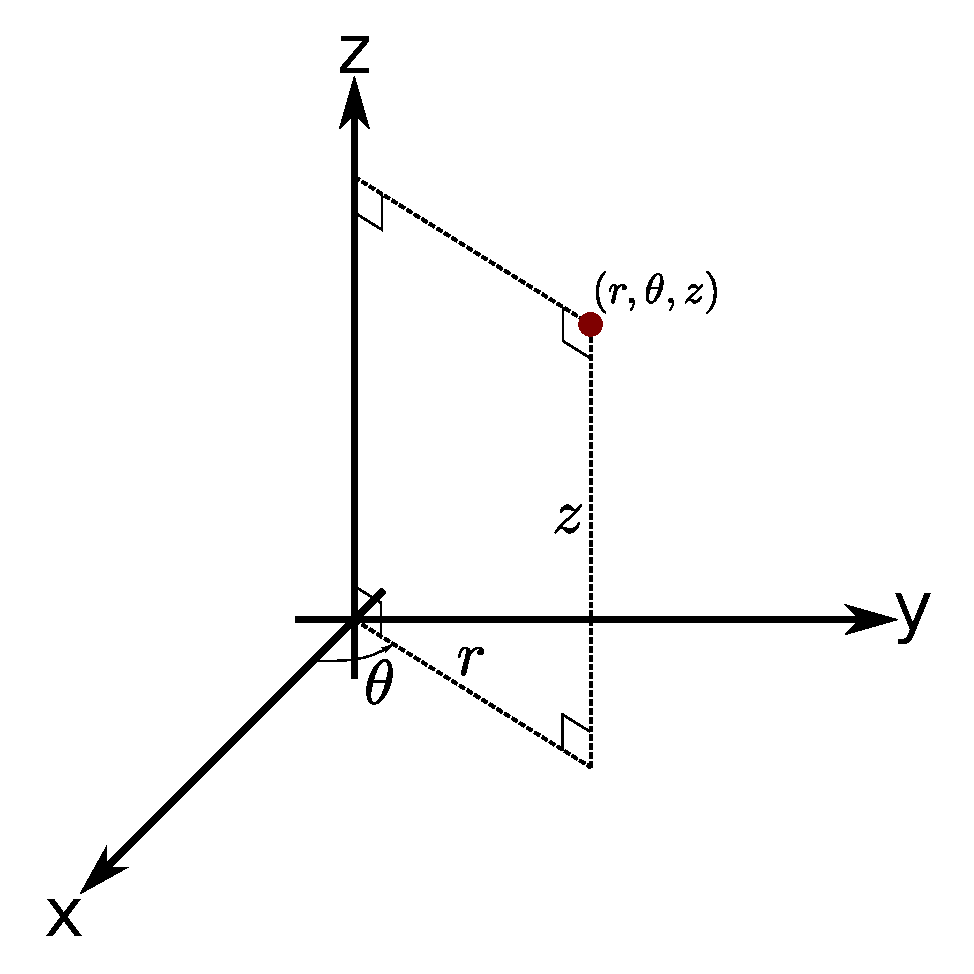
\includegraphics[width = 0.5\textwidth]{Coordinate_systems/cylindrical_coordinates}
}
\end{tabular}

\begin{itemize}
\item Given a multi-path \(\mathbf{J} = \begin{bmatrix} J_\rho \\ J_\phi \\ J_z \end{bmatrix}\) and a multi-surface \(\mathbf{F} = \begin{bmatrix} F_\rho \\ F_\phi \\ F_z \end{bmatrix}\), then the intersection is the multi-point:

\[\mathbf{J} \bullet \mathbf{F} = \begin{bmatrix} J_\rho \\ J_\phi \\ J_z \end{bmatrix} \bullet \begin{bmatrix} F_\rho \\ F_\phi \\ F_z \end{bmatrix} = J_\rho F_\rho + J_\phi F_\phi + J_z F_z\]
%%%
\item Given multi-surfaces \(\mathbf{F} = \begin{bmatrix} F_x \\ F_y \\ F_z \end{bmatrix}\) and \(\mathbf{G} = \begin{bmatrix} G_x \\ G_y \\ G_z \end{bmatrix}\), then the intersection is the multi-path:

\[\mathbf{F} \times \mathbf{G} = \begin{bmatrix} F_\rho \\ F_\phi \\ F_z \end{bmatrix} \times \begin{bmatrix} G_\rho \\ G_\phi \\ G_z \end{bmatrix}
 = \begin{bmatrix} F_\phi G_z - F_z G_\phi \\ F_z G_\rho - F_\rho G_z \\ F_\rho G_\phi - F_\phi G_\rho \end{bmatrix}\]
%%%
\item The endpoints of multi-path \(\mathbf{J} = \begin{bmatrix} J_\rho \\ J_\phi \\ J_z \end{bmatrix}\) is the multi-point:

\[\nabla \bullet \mathbf{J} = \nabla \bullet \begin{bmatrix} J_\rho \\ J_\phi \\ J_z \end{bmatrix} = \frac{1}{\rho}\left(\frac{\partial}{\partial \rho}(\rho \cdot J_\rho) + \frac{\partial}{\partial \phi}(J_\phi) + \frac{\partial}{\partial z}(\rho \cdot J_z)\right)\]
%%%
\item The counterclockwise boundary of multi-surface \(\mathbf{F} = \begin{bmatrix} F_\rho \\ F_\phi \\ F_z \end{bmatrix}\) is the multi-path:

\[\nabla \times \mathbf{F} = \nabla \times \begin{bmatrix} F_\rho \\ F_\phi \\ F_z \end{bmatrix} = \begin{bmatrix} \frac{1}{\rho}\left(\frac{\partial}{\partial \phi}(F_z) - \frac{\partial}{\partial z}(\rho \cdot F_\phi) \right) \\ \frac{\partial}{\partial z}(F_\rho) - \frac{\partial}{\partial \rho}(F_z) \\ \frac{1}{\rho}\left(\frac{\partial}{\partial \rho}(\rho \cdot F_\phi) - \frac{\partial}{\partial \phi}(F_\rho)\right) \end{bmatrix}\]
%%%
\item The inwards oriented surface of multi-volume \(U\) is the multi-surface:

\[\nabla U = \begin{bmatrix} \frac{\partial}{\partial \rho}(U) \\ \frac{1}{\rho}\frac{\partial}{\partial \phi}(U) \\ \frac{\partial}{\partial z}(U) \end{bmatrix}\]
\end{itemize}




\subsection{Spherical coordinates}

\begin{tabular}{cc}
\parbox{0.5\textwidth}{
The 3 coordinates used in {\bf spherical coordinates} are \(c_1 = r\), \(c_2 = \theta\), and \(c_3 = \phi\) (Here \(\theta\) is a coordinate and does not refer to the vertex nodes from the lattice grid.). Coordinate \(r\) is the distance from the origin. Coordinate \(\theta\) is the angle with the \(z\) axis (see the image on the right). Coordinate \(\phi\) is the longitudinal coordinate, the same \(\phi\) coordinate from cylindrical coordinates.

If \((r, \theta, \phi)\) are the coordinates of a lattice vertex, then the dimensions of the cell prism at \((r,\theta,\phi)\) are respectively:
\(1 \cdot \Delta r\); \(r \cdot \Delta\theta\); and \(r\sin\theta \cdot \Delta\phi\)

When \(\Delta\theta\) or \(\Delta\phi\) is large, the cell is not a prism, but has a curve as appears on the right. When \(\Delta\theta\) and \(\Delta\phi\) are infinitely small however as is being assumed, then the cell becomes a rectangular prism.

From these dimensions, the following can be derived:
} & \parbox{0.5\textwidth}{
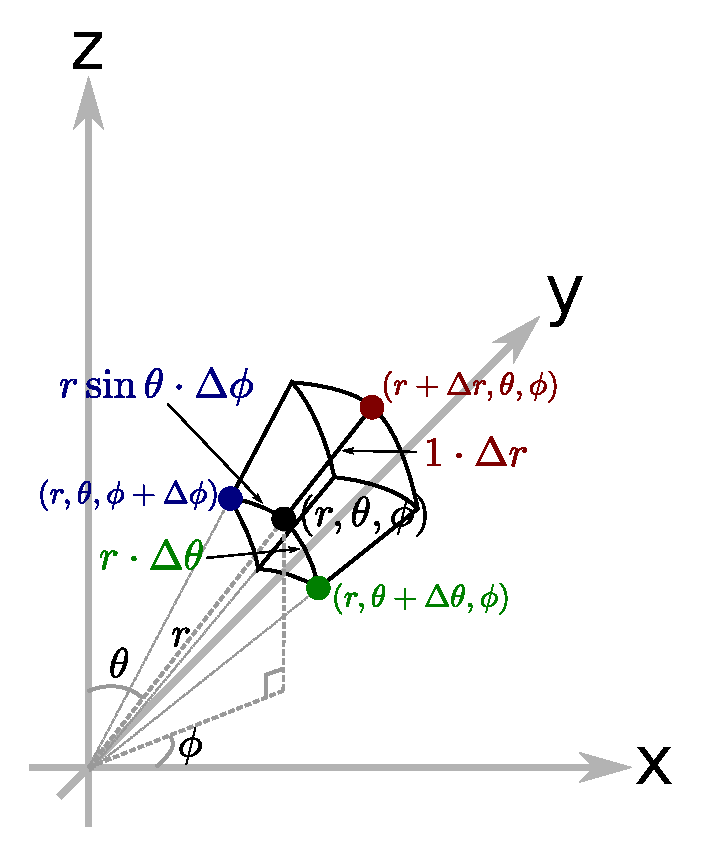
\includegraphics[width = 0.5\textwidth]{Coordinate_systems/spherical_coordinates}
}
\end{tabular}

\begin{itemize}
\item Given a multi-path \(\mathbf{J} = \begin{bmatrix} J_r \\ J_\theta \\ J_\phi \end{bmatrix}\) and a multi-surface \(\mathbf{F} = \begin{bmatrix} F_r \\ F_\theta \\ F_\phi \end{bmatrix}\), then the intersection is the multi-point:

\[\mathbf{J} \bullet \mathbf{F} = \begin{bmatrix} J_r \\ J_\theta \\ J_\phi \end{bmatrix} \bullet \begin{bmatrix} F_r \\ F_\theta \\ F_\phi \end{bmatrix} = J_r F_r + J_\theta F_\theta + J_\phi F_\phi\]
%%%
\item Given multi-surfaces \(\mathbf{F} = \begin{bmatrix} F_r \\ F_\theta \\ F_\phi \end{bmatrix}\) and \(\mathbf{G} = \begin{bmatrix} G_r \\ G_\theta \\ G_\phi \end{bmatrix}\), then the intersection is the multi-path:

\[\mathbf{F} \times \mathbf{G} = \begin{bmatrix} F_r \\ F_\theta \\ F_\phi \end{bmatrix} \times \begin{bmatrix} G_r \\ G_\theta \\ G_\phi \end{bmatrix}
 = \begin{bmatrix} F_\theta G_\phi - F_\phi G_\theta \\ F_\phi G_r - F_r G_\phi \\ F_r G_\theta - F_\theta G_r \end{bmatrix}\]
%%%
\item The endpoints of multi-path \(\mathbf{J} = \begin{bmatrix} J_r \\ J_\theta \\ J_\phi \end{bmatrix}\) is the multi-point:

\[\nabla \bullet \mathbf{J} = \nabla \bullet \begin{bmatrix} J_r \\ J_\theta \\ J_\phi \end{bmatrix} = \frac{1}{r^2 \sin\theta}\left(\frac{\partial}{\partial r}(r^2 \sin\theta \cdot J_r) + \frac{\partial}{\partial \theta}(r \sin\theta \cdot J_\theta) + \frac{\partial}{\partial \phi}(r \cdot J_\phi)\right)\]
%%%
\item The counterclockwise boundary of multi-surface \(\mathbf{F} = \begin{bmatrix} F_r \\ F_\theta \\ F_\phi \end{bmatrix}\) is the multi-path:

\[\nabla \times \mathbf{F} = \nabla \times \begin{bmatrix} F_r \\ F_\theta \\ F_\phi \end{bmatrix} = \begin{bmatrix} 
\frac{1}{r^2\sin\theta}\left(\frac{\partial}{\partial \theta}(r\sin\theta \cdot F_\phi) - \frac{\partial}{\partial \phi}(r \cdot F_\theta) \right) \\ 
\frac{1}{r\sin\theta}\left(\frac{\partial}{\partial \phi}(F_r) - \frac{\partial}{\partial r}(r\sin\theta \cdot F_\phi)\right) \\ 
\frac{1}{r}\left(\frac{\partial}{\partial r}(r \cdot F_\theta) - \frac{\partial}{\partial \theta}(F_r)\right) \end{bmatrix}\]
%%%
\item The inwards oriented surface of multi-volume \(U\) is the multi-surface:

\[\nabla U = \begin{bmatrix} \frac{\partial}{\partial r}(U) \\ \frac{1}{r}\frac{\partial}{\partial \theta}(U) \\ \frac{1}{r\sin\theta}\frac{\partial}{\partial \phi}(U) \end{bmatrix}\]
\end{itemize}



%\subsection*{``Toroidal" coordinates}



\section{Summary}

\begin{itemize}
%%%%%
\item Consider a multi-point that is quantified by the function \(\rho(\mathbf{q})\). The weight assigned to the lattice node \(\theta_{(k_1,k_2,k_3)}\) belonging to the cell that contains \(\mathbf{q}\), is: 
\[w_{\theta} = \rho(\mathbf{q}) \cdot (V \Delta c_1 \Delta c_2 \Delta c_3)\]
%%%%%
\item Consider a multi-path that is quantified by the vector-valued function \(\mathbf{J}(\mathbf{q}) = \begin{bmatrix} J_1(\mathbf{q}) \\ J_2(\mathbf{q}) \\ J_3(\mathbf{q}) \end{bmatrix}\). For each \(i = 1,2,3\), the weight assigned to the lattice edge \(\alpha_{i, (k_1,k_2,k_3)}\) belonging to the cell that contains \(\mathbf{q}\), is:      
\[w_{\alpha,i} = J_i(\mathbf{q}) \cdot (B_i \Delta c_{i+1} \Delta c_{i+2})\]
%%%%%
\item Consider a multi-surface that is quantified by the vector-valued function \(\mathbf{F}(\mathbf{q}) = \begin{bmatrix} F_1(\mathbf{q}) \\ F_2(\mathbf{q}) \\ F_3(\mathbf{q}) \end{bmatrix}\). For each \(i = 1,2,3\), the weight assigned to the lattice tile \(\sigma_{i, (k_1,k_2,k_3)}\) belonging to the cell that contains \(\mathbf{q}\), is:      
\[w_{\sigma,i} = F_i(\mathbf{q}) \cdot (h_i \Delta c_i)\]
%%%%%
\item Consider a multi-volume that is quantified by the function \(U(\mathbf{q})\). The weight assigned to the lattice cell \(\Omega_{(k_1,k_2,k_3)}\) belonging to the cell that contains \(\mathbf{q}\), is: 
\[w_{\Omega} = U(\mathbf{q})\]
\end{itemize}

From these quantities, the following quantities were derived (the parameter \(\mathbf{q}\) will be omitted for simplicity):

\begin{center}
\begin{tabular}{|m{0.15\textwidth}|m{0.15\textwidth}||m{0.6\textwidth}|}
\hline
Quantity 1 
& 
Quantity 2 
& 
Computed quantity 
\\
\hline
\hline
Path \[\mathbf{J} = \begin{bmatrix} J_1 \\ J_2 \\ J_3 \end{bmatrix}\] 
& 
Surface \[\mathbf{F} = \begin{bmatrix} F_1 \\ F_2 \\ F_3 \end{bmatrix}\] 
& 
Intersection point (general): \[\mathbf{J} \bullet \mathbf{F} = \sum_i \frac{B_i h_i}{V} J_i F_i = \frac{B_1 h_1}{V} J_1 F_1 + \frac{B_2 h_2}{V} J_2 F_2 + \frac{B_3 h_3}{V} J_3 F_3\]  
\\
&
&
Intersection point (orthogonal): \[\mathbf{J} \bullet \mathbf{F} = \sum_i J_i F_i = J_1 F_1 + J_2 F_2 + J_3 F_3\] 
\\
\hline
Surface \[\mathbf{F} = \begin{bmatrix} F_1 \\ F_2 \\ F_3 \end{bmatrix}\] 
& 
Surface \[\mathbf{G} = \begin{bmatrix} G_1 \\ G_2 \\ G_3 \end{bmatrix}\] 
& 
Intersection path (general): 
\[\mathbf{F} \times \mathbf{G} = \left[i : \frac{h_{i+1} h_{i+2}}{B_i} (F_{i+1} G_{i+2} - F_{i+2} G_{i+1}) \right]\]
\[= \begin{bmatrix} \frac{h_2 h_3}{B_1} (F_2 G_3 - F_3 G_2) \\ \frac{h_3 h_1}{B_2} (F_3 G_1 - F_1 G_3) \\ \frac{h_1 h_2}{B_3} (F_1 G_2 - F_2 G_1) \end{bmatrix}\]
\\
&
&
Intersection path (orthogonal): 
\[\mathbf{F} \times \mathbf{G} = \left[i : F_{i+1} G_{i+2} - F_{i+2} G_{i+1} \right]\] 
\[= \begin{bmatrix} F_2 G_3 - F_3 G_2 \\ F_3 G_1 - F_1 G_3 \\ F_1 G_2 - F_2 G_1 \end{bmatrix}\] 
\\
\hline
\end{tabular}
\end{center}


\begin{center}
\begin{tabular}{|m{0.3\textwidth}||m{0.6\textwidth}|}
\hline
Quantity 
& 
Computed quantity 
\\
\hline
\hline  
Path \[\mathbf{J} = \begin{bmatrix} J_1 \\ J_2 \\ J_3 \end{bmatrix}\] 
& 
Endpoints (general): 
\[\nabla \bullet \mathbf{J} = \frac{1}{V}\sum_i \frac{\partial}{\partial c_i}(B_i J_i)\] 
\[= \frac{1}{V}\left(\frac{\partial}{\partial c_1}(B_1 J_1) + \frac{\partial}{\partial c_2}(B_2 J_2) + \frac{\partial}{\partial c_3}(B_3 J_3)\right)\] 
\\ 
&
Endpoints (orthogonal): 
\[\nabla \bullet \mathbf{J} = \frac{1}{l_1 l_2 l_3}\sum_i \frac{\partial}{\partial c_i}(l_{i+1} l_{i+2} J_i)\] 
\[= \frac{1}{l_1 l_2 l_3}\left(\frac{\partial}{\partial c_1}(l_2 l_3 J_1) + \frac{\partial}{\partial c_2}(l_3 l_1 J_2) + \frac{\partial}{\partial c_3}(l_1 l_2 J_3)\right)\] 
\\
\hline
\end{tabular}
\end{center}

\begin{center}
\begin{tabular}{|m{0.3\textwidth}||m{0.6\textwidth}|}
\hline
Surface \[\mathbf{F} = \begin{bmatrix} F_1 \\ F_2 \\ F_3 \end{bmatrix}\] 
& 
Boundary (general):
\[\nabla \times \mathbf{F} = \left[i : \frac{1}{B_i}\left(\frac{\partial}{\partial c_{i+1}}(h_{i+2} F_{i+2}) - \frac{\partial}{\partial c_{i+2}}(h_{i+1} F_{i+1})\right)\right]\]
\[= \begin{bmatrix}
\frac{1}{B_1}\left(\frac{\partial}{\partial c_2}(h_3 F_3) - \frac{\partial}{\partial c_3}(h_2 F_2)\right) \\ 
\frac{1}{B_2}\left(\frac{\partial}{\partial c_3}(h_1 F_1) - \frac{\partial}{\partial c_1}(h_3 F_3)\right) \\ 
\frac{1}{B_3}\left(\frac{\partial}{\partial c_1}(h_2 F_2) - \frac{\partial}{\partial c_2}(h_1 F_1)\right) \\
\end{bmatrix}\]
\\
&
Boundary (orthogonal):
\[\nabla \times \mathbf{F} = \left[i : \frac{1}{l_{i+1} l_{i+2}}\left(\frac{\partial}{\partial c_{i+1}}(l_{i+2} F_{i+2}) - \frac{\partial}{\partial c_{i+2}}(l_{i+1} F_{i+1})\right)\right]\]
\[= \begin{bmatrix}
\frac{1}{l_2 l_3}\left(\frac{\partial}{\partial c_2}(l_3 F_3) - \frac{\partial}{\partial c_3}(l_2 F_2)\right) \\ 
\frac{1}{l_3 l_1}\left(\frac{\partial}{\partial c_3}(l_1 F_1) - \frac{\partial}{\partial c_1}(l_3 F_3)\right) \\ 
\frac{1}{l_1 l_2}\left(\frac{\partial}{\partial c_1}(l_2 F_2) - \frac{\partial}{\partial c_2}(l_1 F_1)\right) \\
\end{bmatrix}\]
\\
\hline
\end{tabular}
\end{center}

\begin{center}
\begin{tabular}{|m{0.3\textwidth}||m{0.6\textwidth}|}
\hline
Volume \[U\]
&
Surface (general): 
\[\nabla U = \left[i : \frac{1}{h_i}\frac{\partial}{\partial c_i}(U)\right]
= \begin{bmatrix}
\frac{1}{h_1}\frac{\partial}{\partial c_1}(U) \\ 
\frac{1}{h_2}\frac{\partial}{\partial c_2}(U) \\ 
\frac{1}{h_3}\frac{\partial}{\partial c_3}(U)
\end{bmatrix}\]
\\ 
&
Surface (orthogonal): 
\[\nabla U = \left[i : \frac{1}{l_i}\frac{\partial}{\partial c_i}(U)\right]
= \begin{bmatrix}
\frac{1}{l_1}\frac{\partial}{\partial c_1}(U) \\ 
\frac{1}{l_2}\frac{\partial}{\partial c_2}(U) \\ 
\frac{1}{l_3}\frac{\partial}{\partial c_3}(U)
\end{bmatrix}\]
\\
\hline 
\end{tabular}
\end{center}








